\chapter{Architecture and Technology}

This chapter is about introducing different software architectures and 
technologies that are used to build web applications. \index{software architecture}
The first section discusses the advantages and disadvantages of web
 applications versus desktop applications. The second part deals with
JavaScript as the primary programming language for web application user interfaces. 
Thereafter we will take a more detailed look into a modern framework for web-based user interfaces called React
and its underlying software architecture Flux.
Complex user interfaces built on React can be further enhanced using a framework called Redux, which will be discussed in the fourth section. And finally we will introduce TensorFlow.js as the key library for machine learning within browsers.  \index{Redux} 
   
  
\section{Software application architectures}
Most software applications fall into one of these
categories:

\begin{itemize}
	\item Desktop application
	\item Web application
	\item App for mobile devices
\end{itemize}

There is a clear trend towards web applications as they come
with two significant benefits:

\begin{itemize}
	\item No installation is required by the end user
	\item The runtime environment (web browser) is usually
	      available on all platforms and standardized
\end{itemize}

This trend is reflected by the popularity of JavaScript as 
the programming language of choice for web applications 
(see Fig. \ref{fig:JSgithub}).

\begin{figure}[ht]
	\centering
	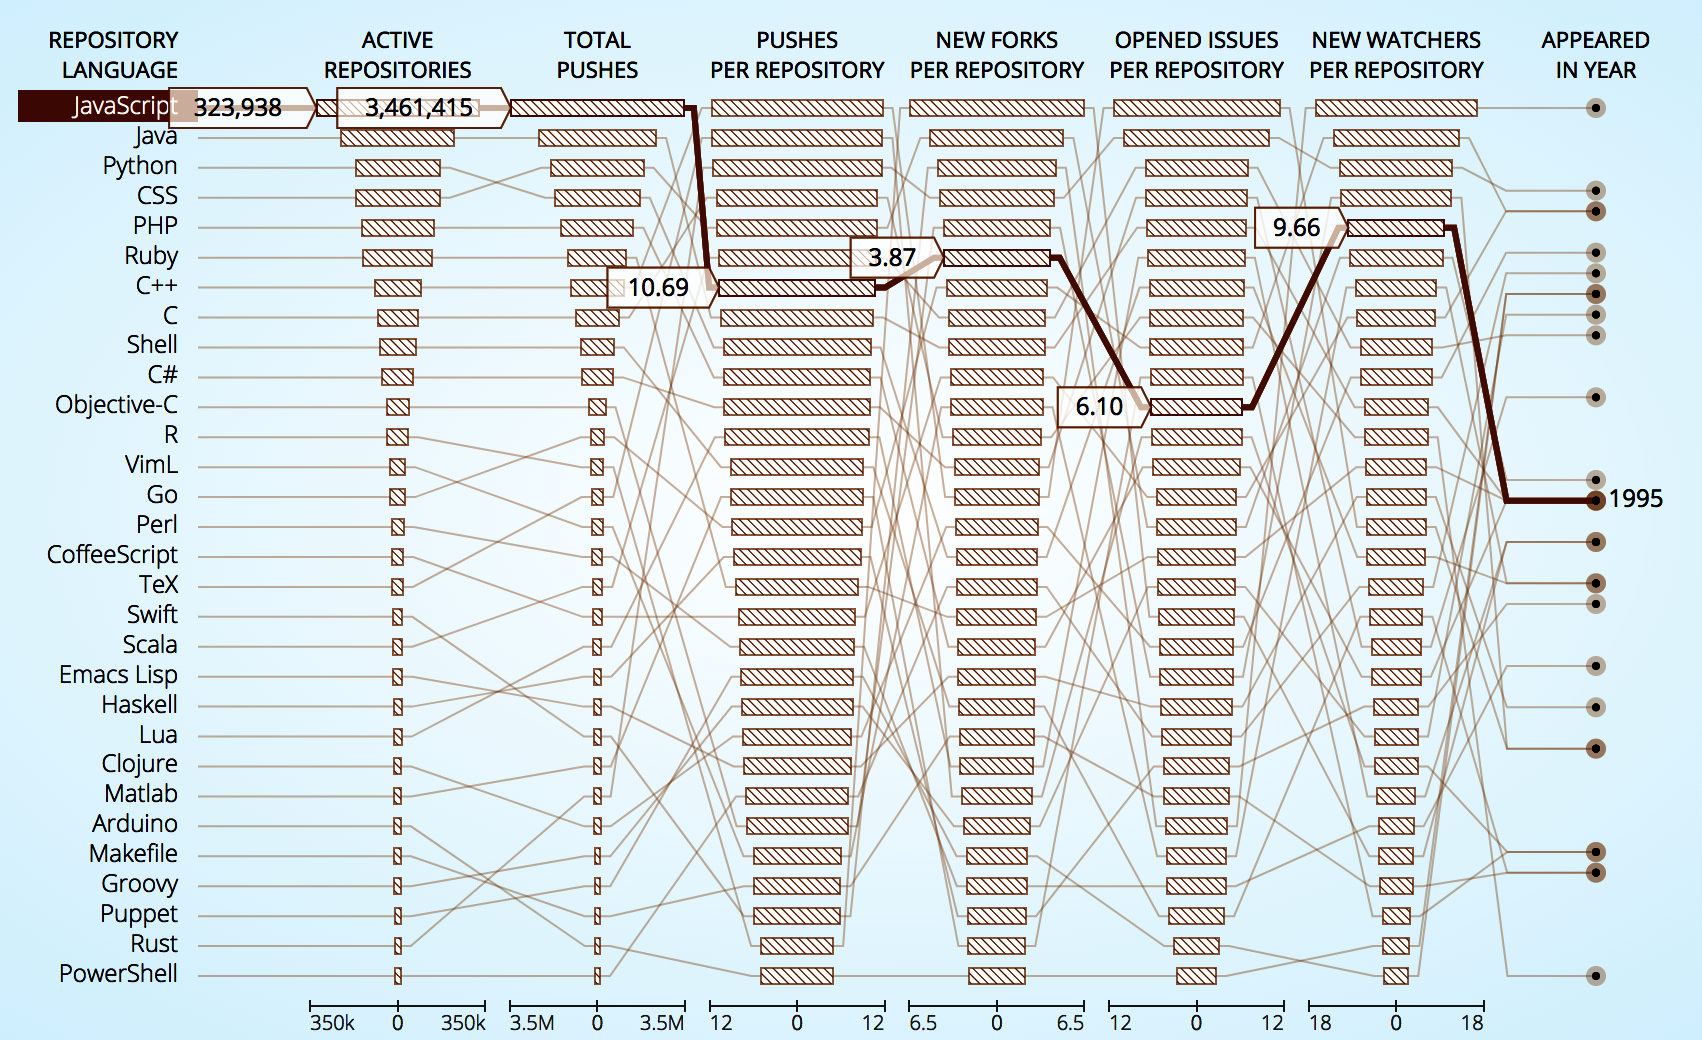
\includegraphics[width=\linewidth]{bilder/grundlagen/jsUsage.png}
	\caption{Numbers of Github repositories using JavaScript 2014 \cite{GitHut}} 
	\label{fig:JSgithub}
\end{figure}

\section{JavaScript}
Today JavaScript is one of the most used programming languages world wide.

JavaScript first appeared in 1995. Originally developed at Netscape
by Brendan Eich under the name of "LiveScript" it had a simple purpose, namely to dynamically manipulate the HTML Document Object Model (DOM) tree in the browser. 
 
At about the same time a company called Sun worked on a programming
language for embedded and mobile devices called Java.   
As Java became increasingly popular,
Netscape considered it a good marketing move to rename its
LiveScript to JavaScript, even though there was little technological
similarity between these two languages.
    
Java is a regular, static, and highly typed programming language.
It runs on a virtual machine and needs to be compiled, whereas the
single threaded JavaScript only runs in a browser and is a script
language. 
  
Both languages have in common a C related syntax and exhibit some 
similarities with regard to naming conventions. While Java is a true
object oriented language, JavaScript has incorporated elements
supporting object oriented programming only over time \cite{Bewersdorff2018ObjektorientierteProgrammierung}. 
  
The JavaScript community considers this language superior for web development. Jeff Attwood, the co-founder of 
the  computer programming question-and-answer website Stack Overflow and Stack Exchange, even said: 
"Any application that can be written in JavaScript, will eventually be written in JavaScript" \cite{Louis2018Java}.
 
\subsection{JavaScript distributed architectures}

Most modern web designs rely on a three-tier architecture (Fig. 
\ref{fig:TT}). The bottom tier is usually a database system, responsible for storing and retrieving data. Typical 
technologies employed here are relational database management systems (RDBMS) and, more recently noSQL database systems like key value stores \cite{GOLL}. 

The second tier is usually responsible for executing the application logic.
The technological base for this layer is Java, .NET, and more recently Node.js.
 
The top most tier is typically responsible for the user interface, but can also contain application logic.
The most widely used technology nowadays is a web browser with JavaScript programs. 

\begin{figure}[H]
	\centering
	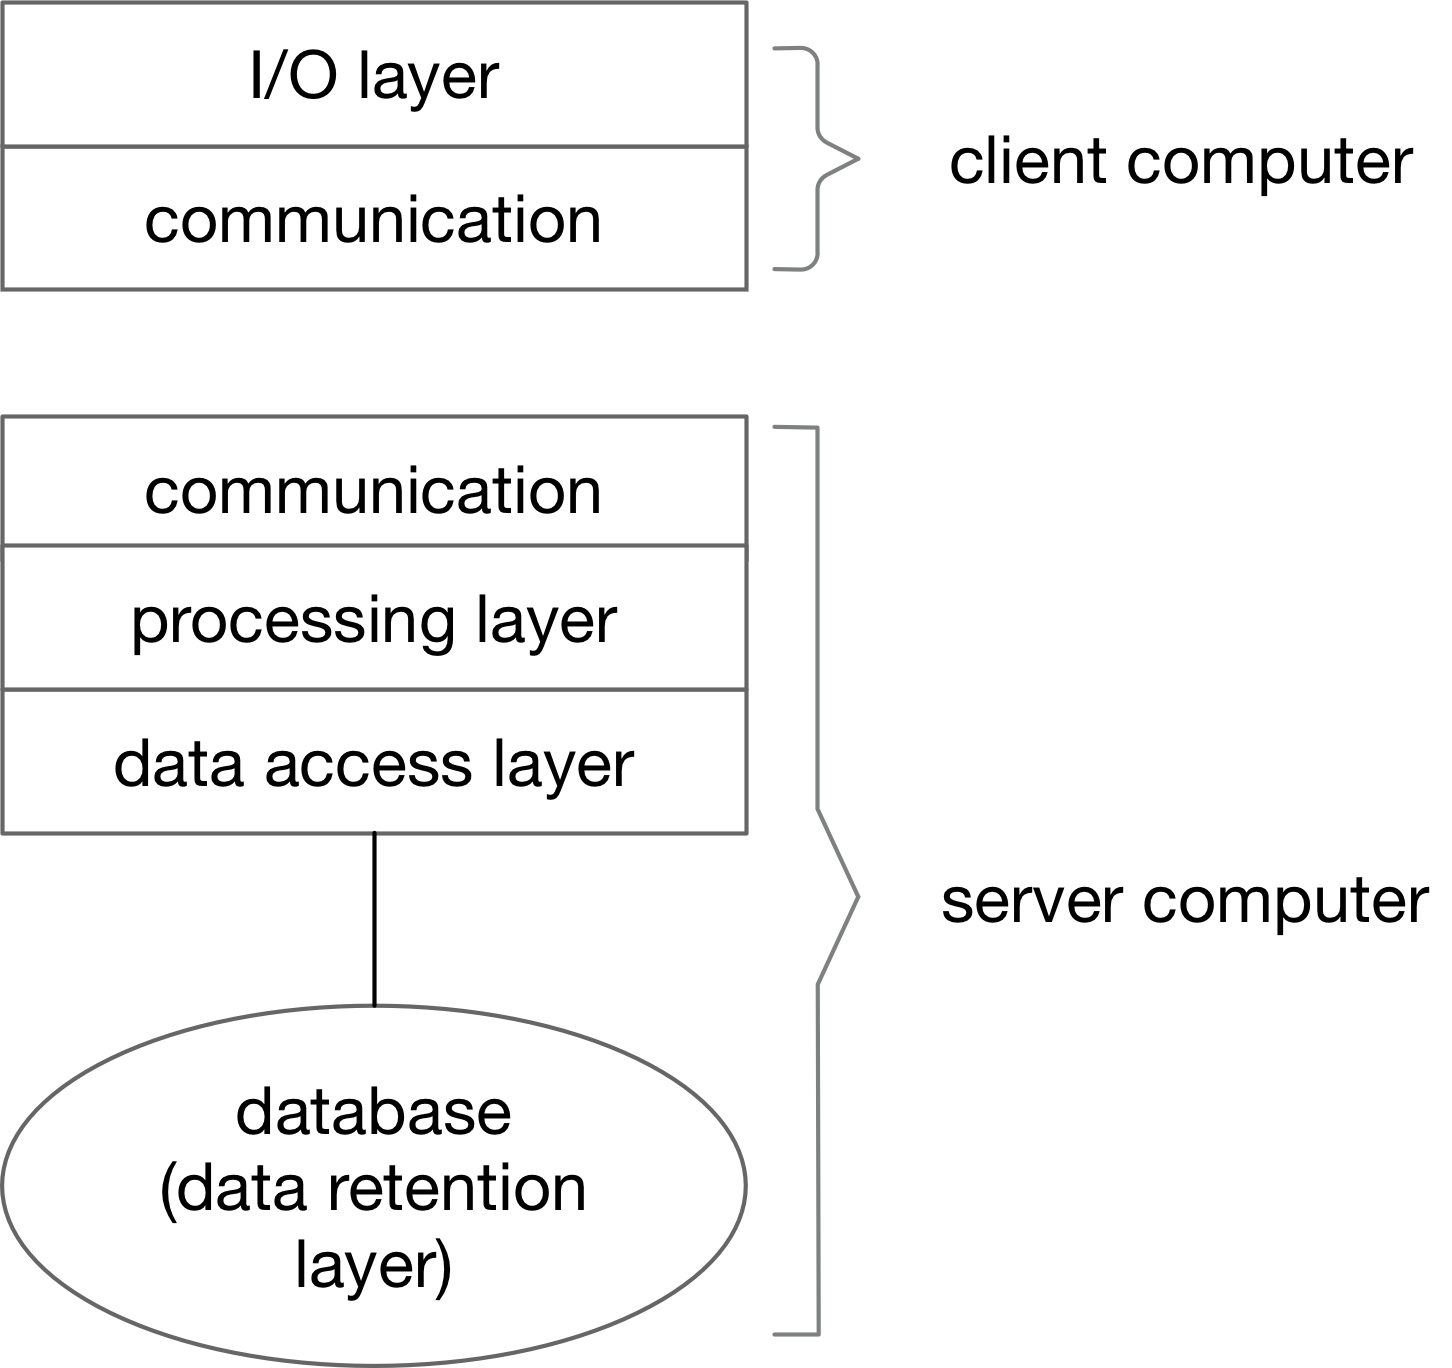
\includegraphics[width=0.5\linewidth]{bilder/grundlagen/Three-Tier.png}
	\caption{Three-Tier architecture \cite{GOLL}}
	\label{fig:TT}
\end{figure}

The three tier architecture requires a wide spectrum of technological know-how:
Know\-ledge about database management systems which is a discipline on its own,
then deep knowledge of the Java or  .NET ecosystem, and knowledge about HTML, 
cascaded style sheets, JavaScript 
and possibly JavaScript frameworks used for the design of the user interface.

To reduce the amount of programming languages to be used some people have advocated 
JavaScript also as a server side language. This has become  popular with the Node.js 
framework which permits JavaScript developers to employ their programming language 
skills on the client side as well as on the server side. 

On the account of type safety, this approach fosters rapid application development.
Using a single language on both sides adds the chance of sharing modules,
thus further reducing development time (see Figs. \ref{fig:DS1} and  \ref{fig:DS2}).
This novel approach even affects the job market. Iin the past front-end and back-end developers 
had required different 
skills. This has changed now and people can do full-stack web development with just 
good JavaScript knowledge. 
 

\begin{figure}[H]
	\centering
	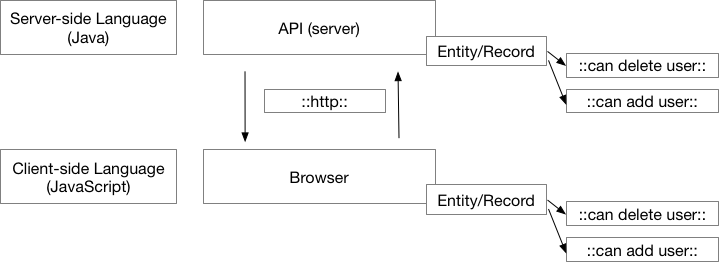
\includegraphics[width=0.8\linewidth]{bilder/grundlagen/Entity1.png}
	\caption{Duplication of functionality due to heterogeneous programming languages}
	\label{fig:DS1}
\end{figure}

\begin{figure}[H]
	\centering
	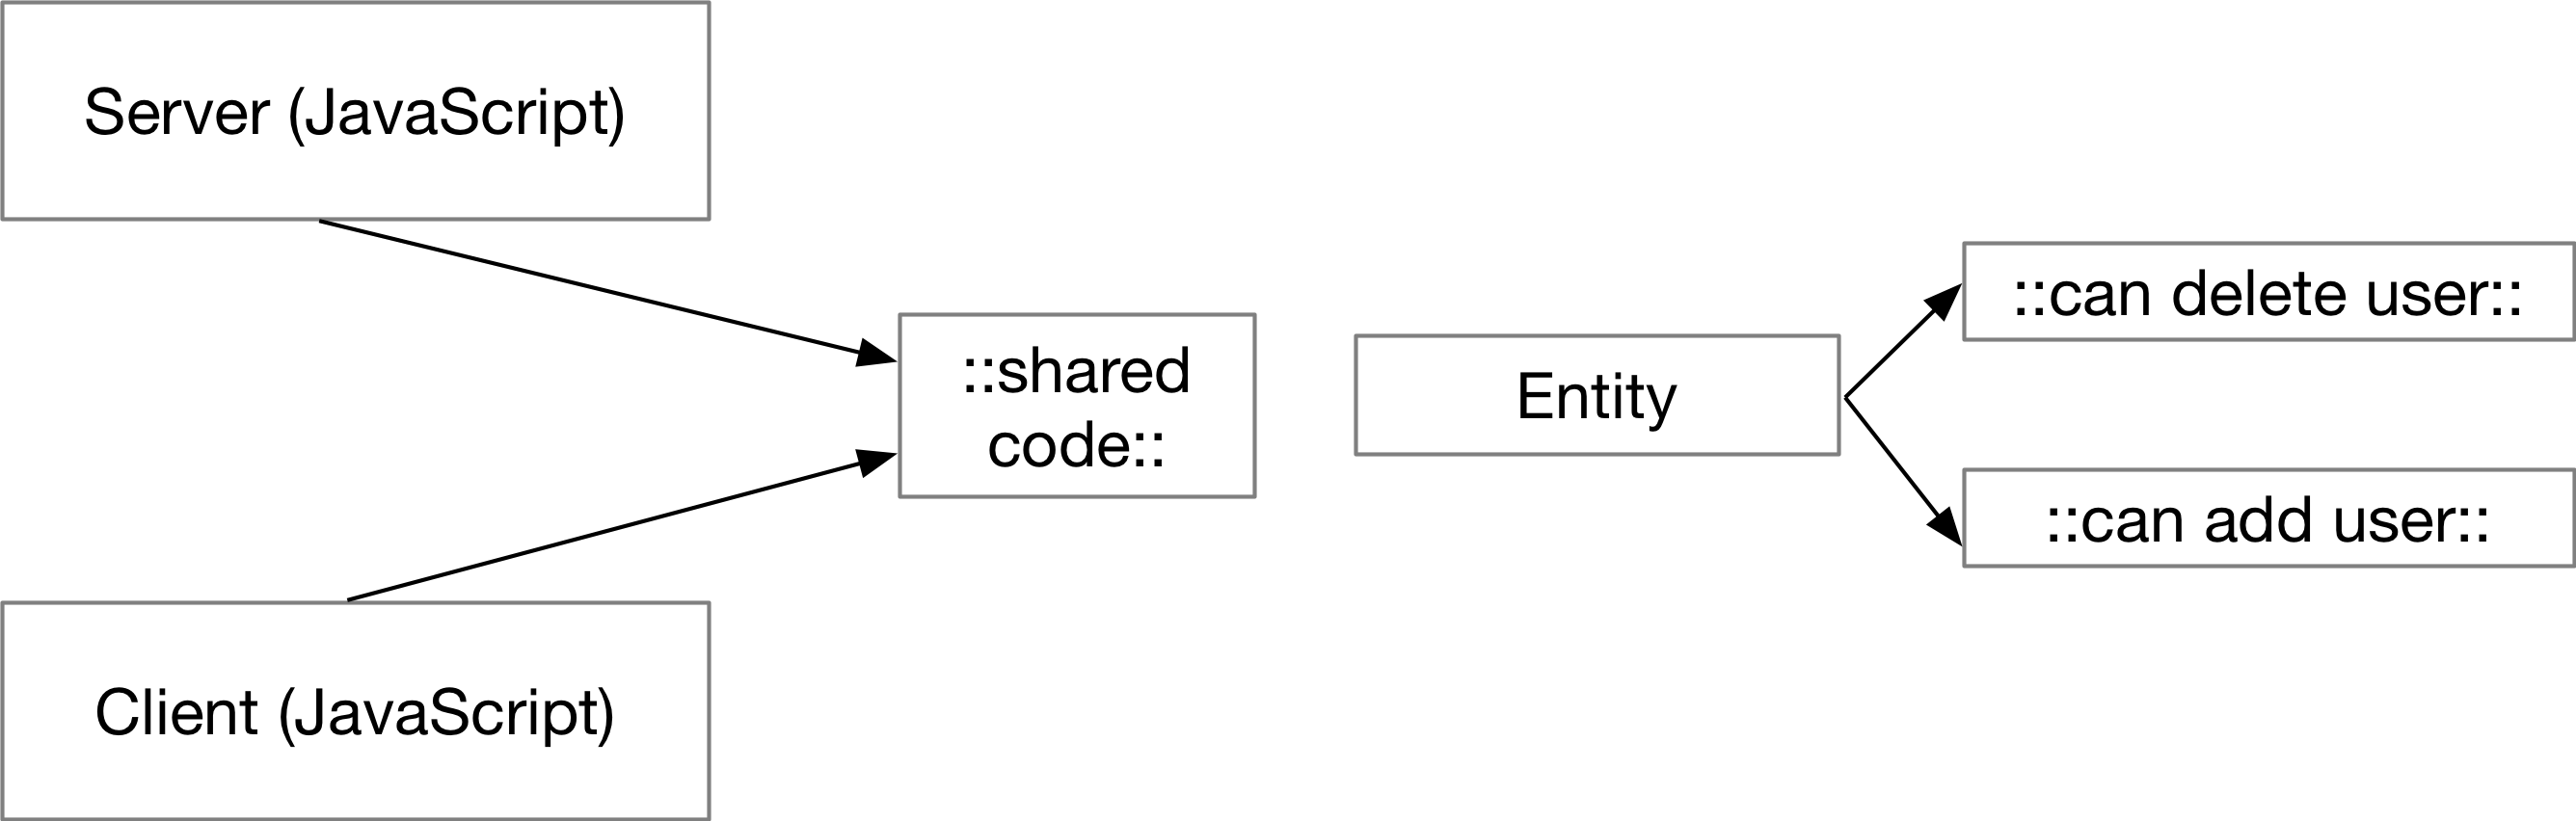
\includegraphics[width=0.8\linewidth]{bilder/grundlagen/Entity2.png}
	\caption{Reuse of shared modules due to a single language approach}
	\label{fig:DS2}
\end{figure}


\subsection{Multi-Platform support}


It is expensive to develop an application for a number of platforms like Android or iOS for tablets and Windows,
Linux or MacOs for desktop computers. Creating applications for any of these platforms
requires large amounts of platform specific code while little can be shared.
Java has provided a way out of this dilemma with the exception of the popular iOS. 
Apple does not allow Java to run
on their mobile devices.

There exist other cross-platform frameworks like QT. However, they require people to program in C++
which is not the most efficient way to create user interfaces anymore.


With JavaScript developers can take advantage of modern frameworks like React Native or Electron, which make it possible to almost completely code in JavaScript. 

The JavaScript communicates with native components that might be written in Java on
Android, in Objective C on iOS, in CSharp on Windows and so on. A so called "bridge"
(see Fig. \ref{fig:BP}) forwards calls from JavaScript to native components and returns
responses back to the JavaScript part. This facilitates user interfaces to 
have a native look and feel even though they are written in JavaScript \cite{Purewal2014LearningWeb}.

\begin{figure}[H]
	\centering
	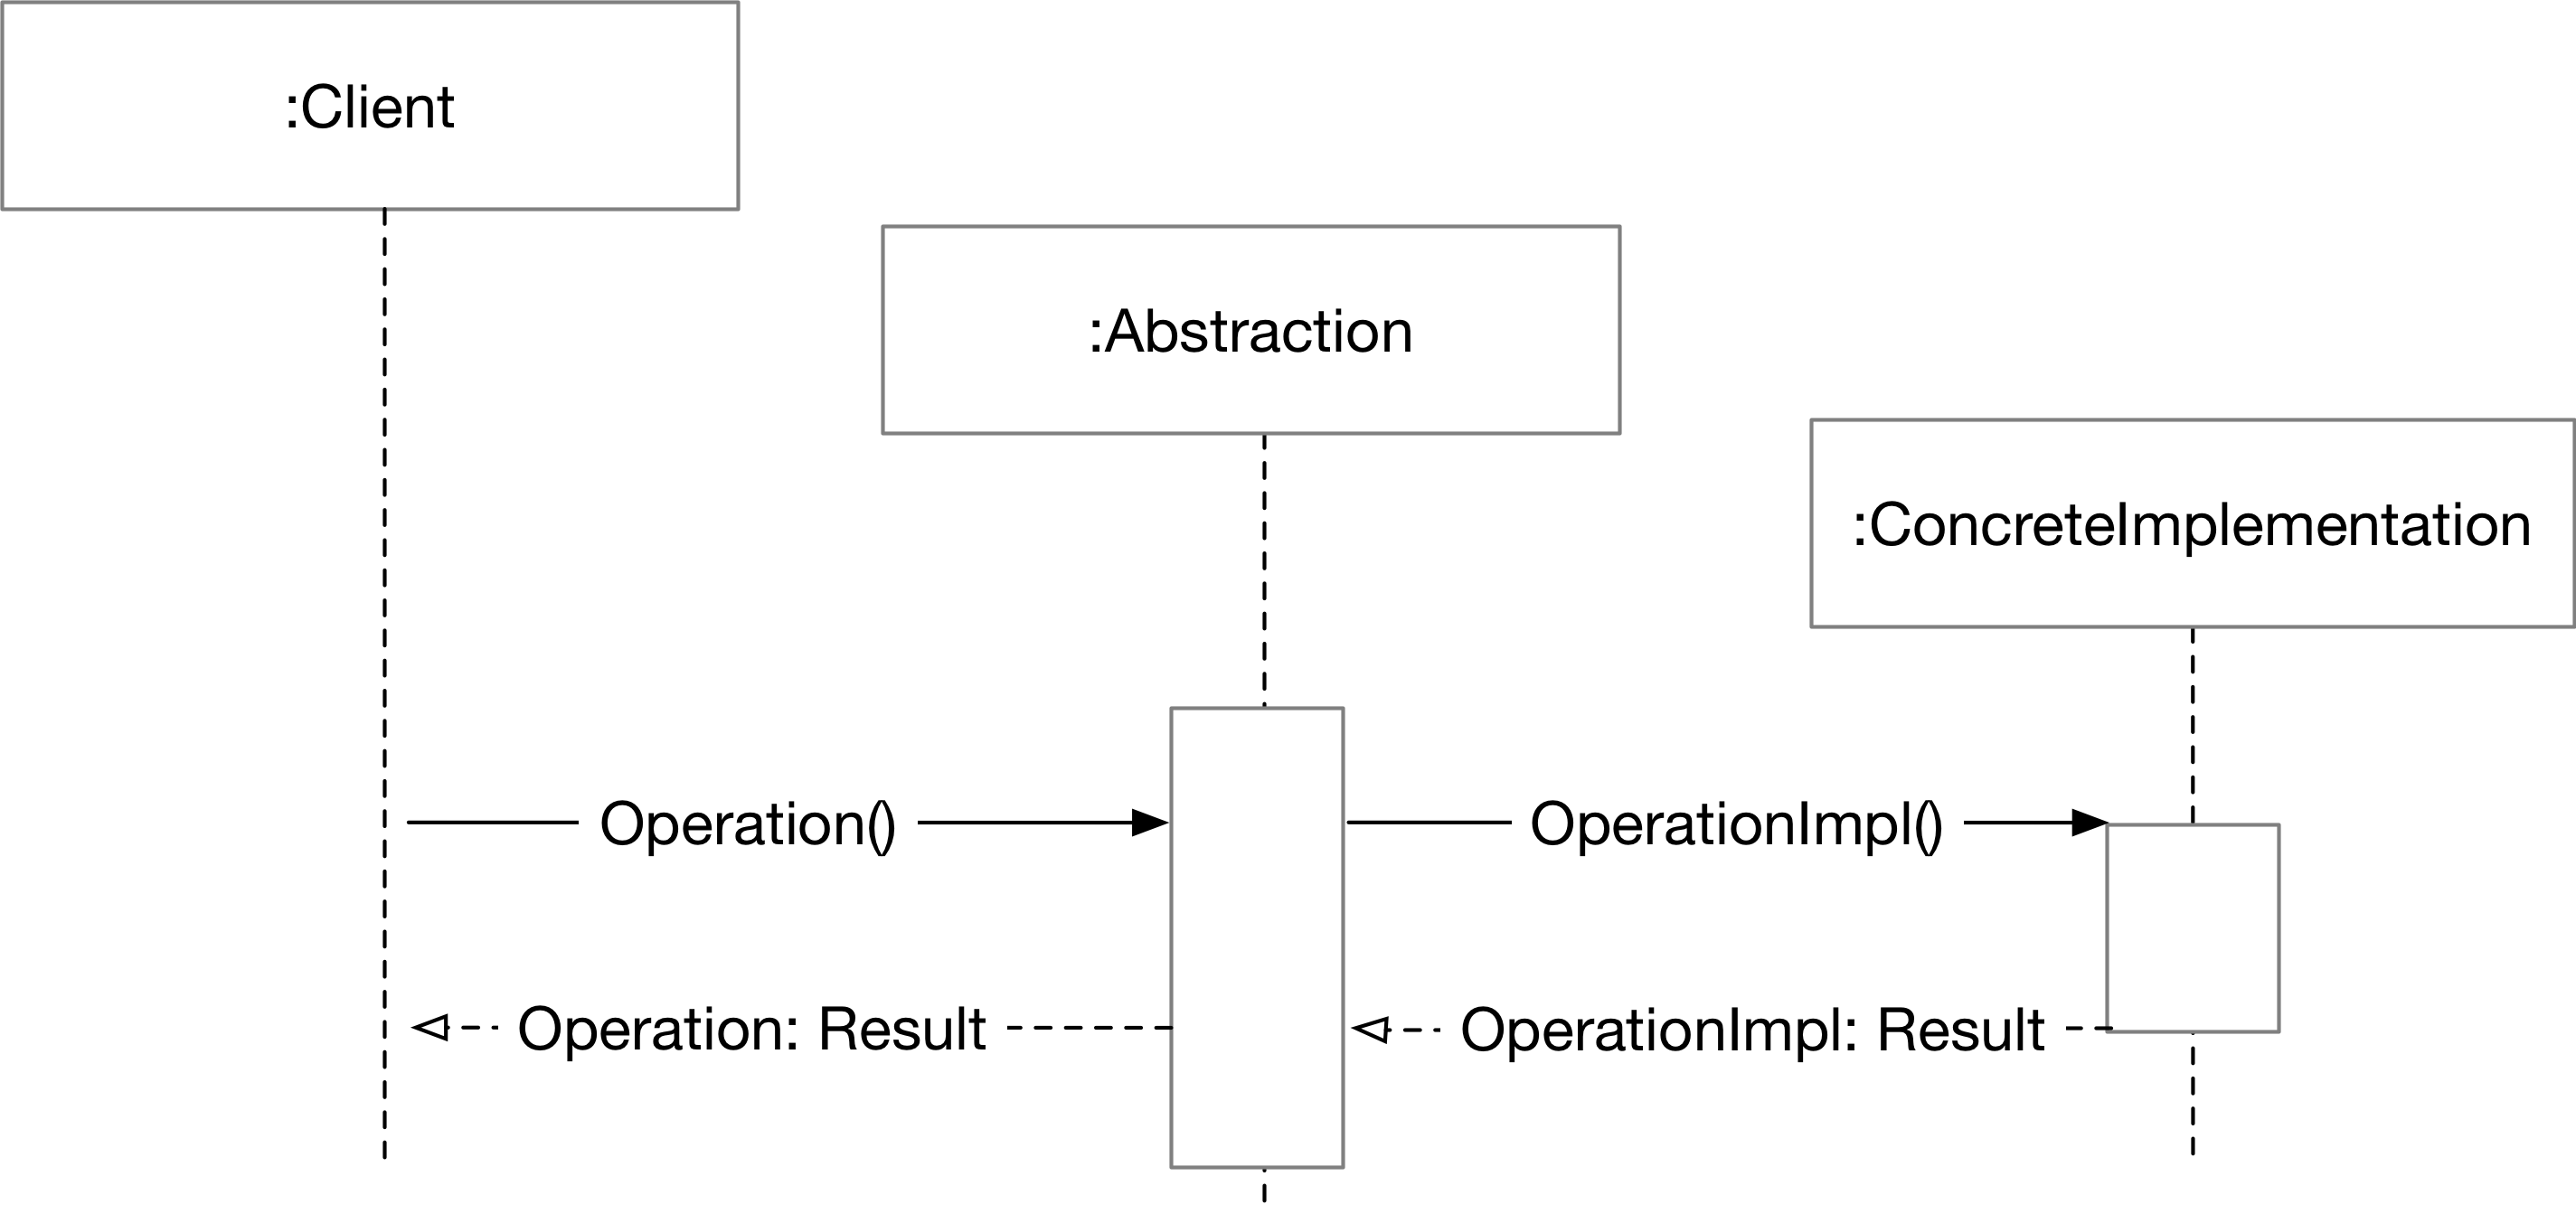
\includegraphics[width=1.0\linewidth]{bilder/grundlagen/BridgePattern.png}
	\caption{Bridge pattern \cite{GOLL}}
	\label{fig:BP}
\end{figure}


\subsection{Single threading and concurrency}

JavaScript is a single threaded programming language with some extension for asynchronous processing.
A JavaScript program may never have an infinite loop, regardless at which level.
This is due to the fact how JavaScript handles concurrency. JavaScript was developed to manipulate the DOM. 
The DOM is a singular structure and it is easily conceivable that changing it from different threads would result in a big mess.
Thus it made no sense to have JavaScript support concurrency.

On the other hand the browser had to interact with remote servers 
which could lead to large delays until a response would have been received.
Blocking the single JavaScript thread with such calls would have lead to
a rather poor user experience, basically blocking 
any user interaction while the browser was waiting for
the servers response.

The designers of JavaScript therefore provided a way to execute outside asynchronous calls
with so called "callbacks".  Every time a function is called in JavaScript, it is put on a call stack.  
Once the function returns 
the result is popped from the stack.  Each function on the stack is executed purely synchronously 
one after the other (see Fig. \ref{fig:CS}).

\begin{figure}[H]
	\centering
	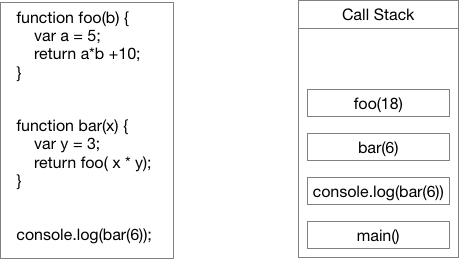
\includegraphics[scale=0.6]{bilder/grundlagen/CallStack.png}
	\caption{Call Stack}
	\label{fig:CS}
\end{figure}

In order to execute code concurrently, JavaScript needs to call the Web API provided by the browser. The web browser runs on a multi threaded operating system so it fully supports concurrency. 

The Web API is called with the function that needs to be executed,  and a callback function.
The callback function is called by the asynchronous function when it finishes execution. 
It is mandatory to provide a callback with each asynchronous function call.

Once the thread executing the asynchronous function is finished it passes the callback to the so 
called "callback queue".
The callback queue is a simple list containing all callbacks waiting for execution.

An event loop continuously checks if the call stack is empty. As soon as that is the case the first 
callback function from the callback queue is placed on the callstack and executed synchronously. 
This decoupling of the caller from the response allows JavaScript to do other things while waiting 
for asynchronous operations to complete and their callbacks to fire (see Fig. \ref{fig:CC}).


\begin{figure}[H]
	\centering
	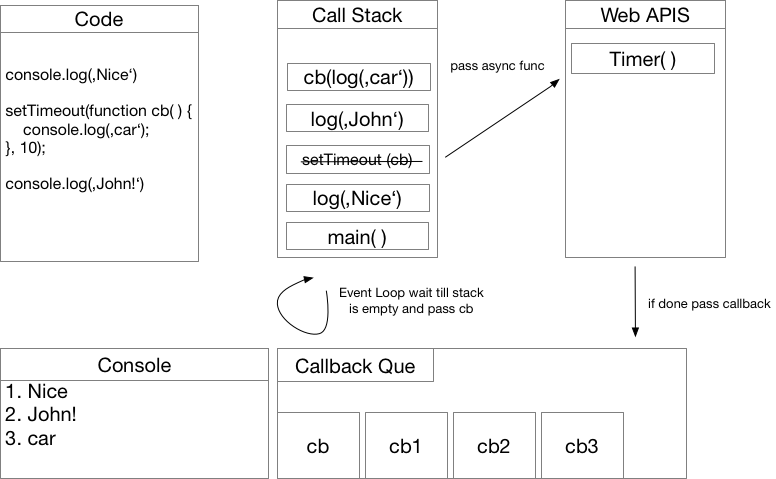
\includegraphics[width=1.0\linewidth]{bilder/grundlagen/Concurrency.png}
	\caption{Concurrency in JavaScript}
	\label{fig:CC}
\end{figure}

\subsection{Functional programming paradigm}

JavaScript is a functional programming language, that is it is possible to 
pass functions as parameters and to return
functions as results. In the functional programming paradigm the return value of a function shall not depend on global variables or state variables, it shall purely depend on its input arguments (see Fig. \ref{fig:FP})\cite{Steyer2014JavaScript}.

In the latest releases of the JavaScript standard provisions have been made to better support the object
oriented paradigm.

\begin{figure}[H]
	\centering
	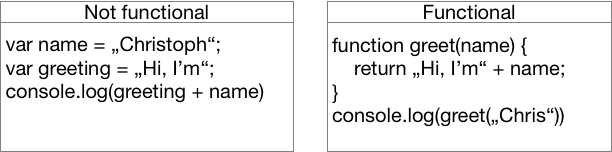
\includegraphics[scale=0.6]{bilder/grundlagen/fp.png}
	\caption{Imperative and functional programming}
	\label{fig:FP}
\end{figure}

In JavaScript it is possible to define functions as part of higher-order functions  \ref{fig:HF}. 

\begin{figure}[H]
	\centering
	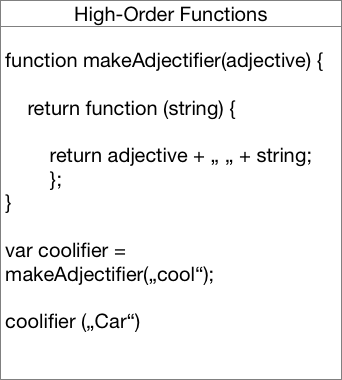
\includegraphics[scale=0.6]{bilder/grundlagen/fp1.png}
	\caption{High-order functions}
	\label{fig:HF}
\end{figure}

\section{Software patterns for web-development}

\subsection{The classic model view controller model}

For a long time it was best practice to use the model view controller (MVC) architectural 
pattern for implementing user interfaces. In this pattern, the model stores the data 
presented in one or more views. In simple systems the model may contain some
 business logic (see Fig \ref{fig:MVC}).

The controller controls the model and view state, based on user input.
For example it activates or deactivates buttons.
 It also transforms events caused by user actions into method calls of the model 
\cite{GOLL}. 
 
The view serves to present model data to the user. There can be many views on the 
same model data. In case of a model data change all views are updated. 
Beside presenting model data the view also provides interactive elements.

The model shall be independent of views and controllers. In case the model changes, 
the controller may inform the views (passive model). With the alternative active model 
implementation, the model informs the views of any change.

\begin{figure}[H]
	\centering
	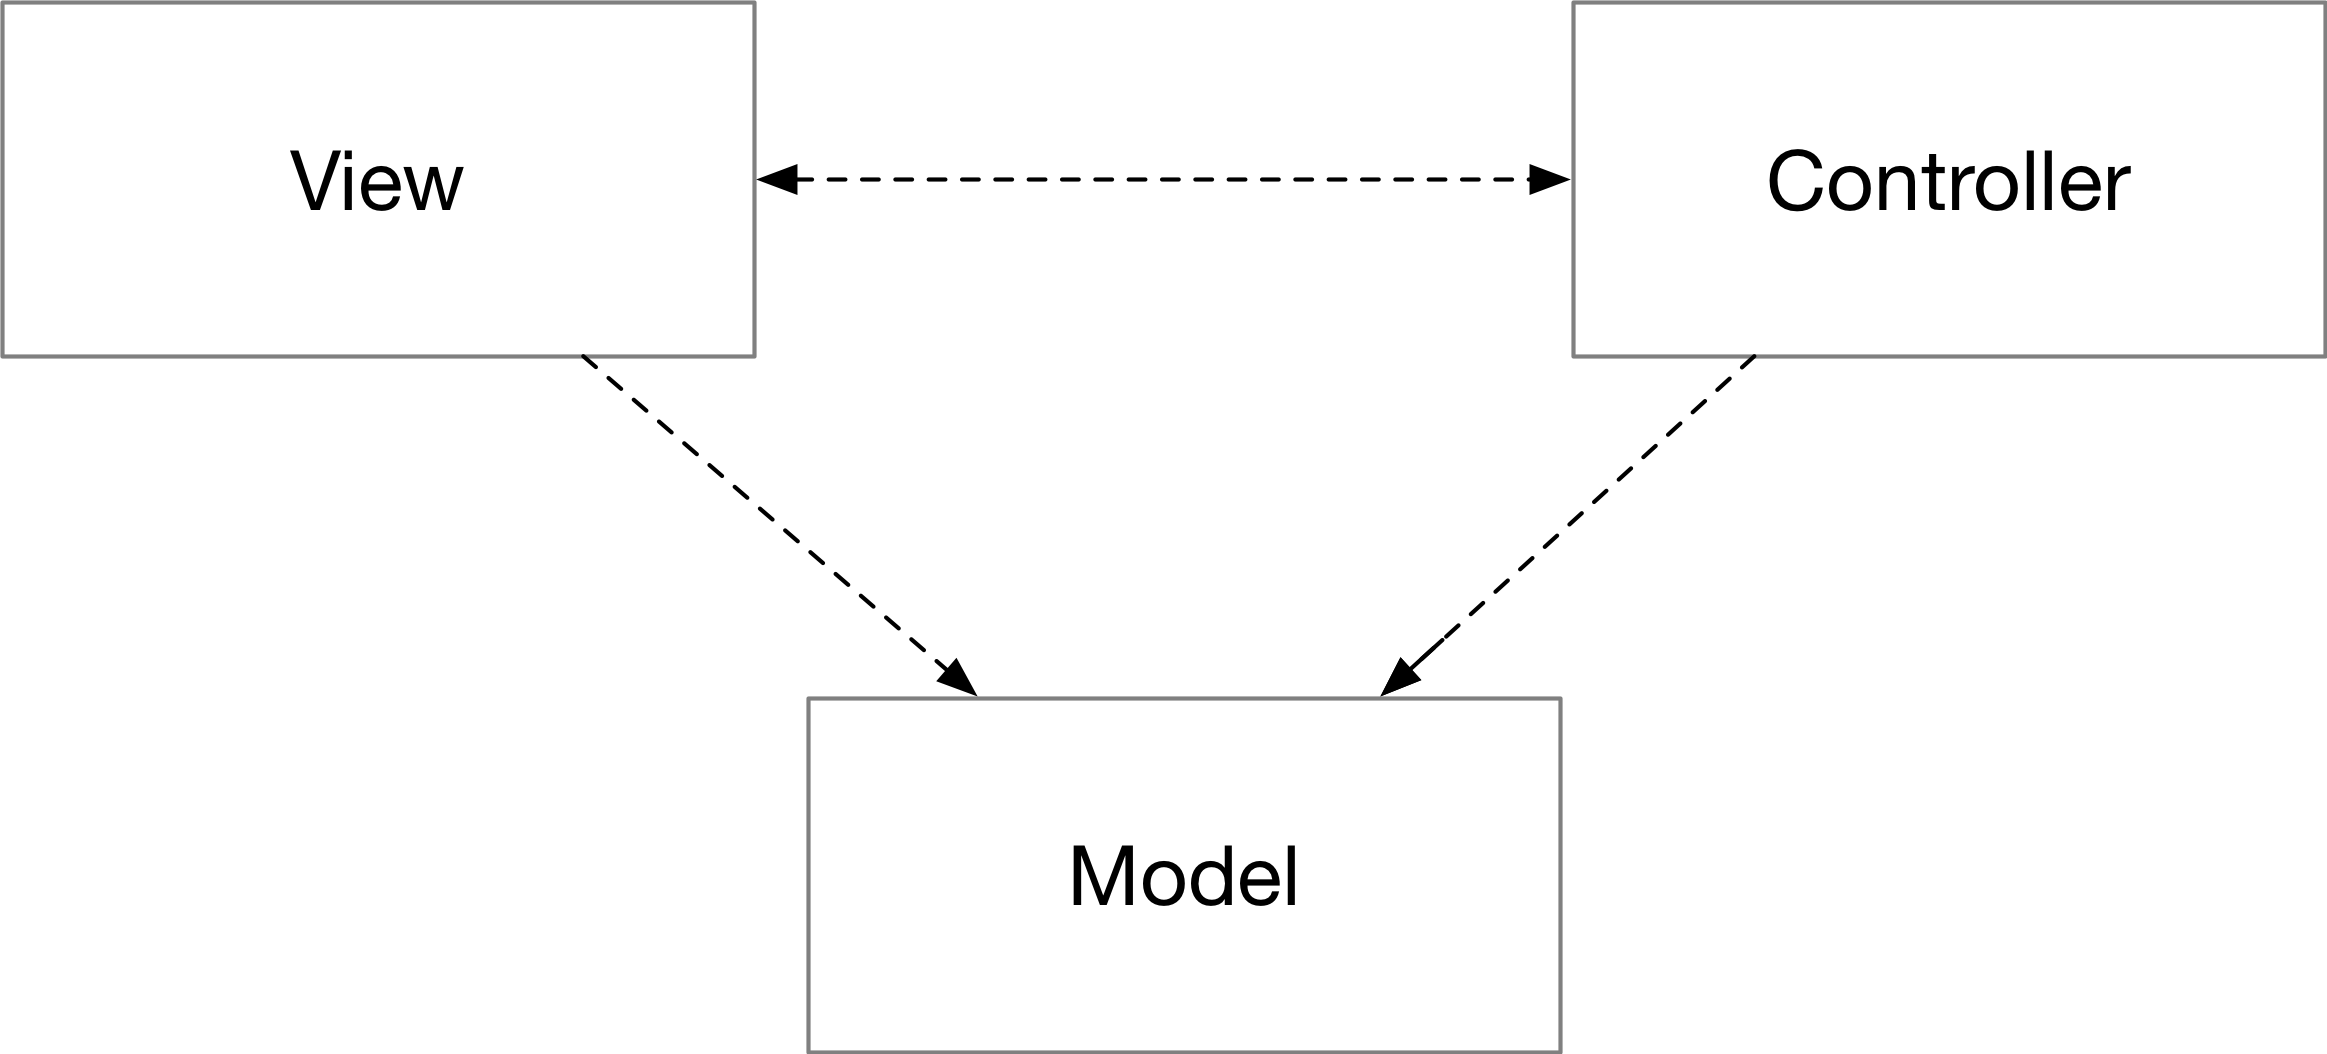
\includegraphics[scale=0.6]{bilder/grundlagen/MVC.png}
	\caption{MVC  software architecture  \cite{GOLL}}
	\label{fig:MVC}
\end{figure}

The so called principle "separation of concerns" makes it easier to split work and thereby 
makes it easier to maintain code.
A drawback is the increased number of classes and larger complexity.
For example,  changes in the model or the controller affect the whole entity. 
The bidirectional communication in the MVC structure makes it hard to debug.
Changing one entity has a cascading effect across the codebase.

The React framework tries to keep the benefits of the MVC pattern while at the same time 
avoiding some of its disadvantages. To that end it employs a different architecture called
Flux which shall be explained below.

\subsection{Flux}

\subsubsection{Structure and data flow}
The Flux architecture consists of actions, dispatchers, stores and views. In Flux data flows in a single direction.
The unidirectional data flow is central to the Flux concept (see Fig. \ref{fig:FLUX}).
Dispatcher, stores and views are independent nodes with different inputs and outputs. The actions simply consist of objects with the new data. The following sections are inspired by the official Flux guide \cite{Flux}.

\begin{figure}[H]
	\centering
	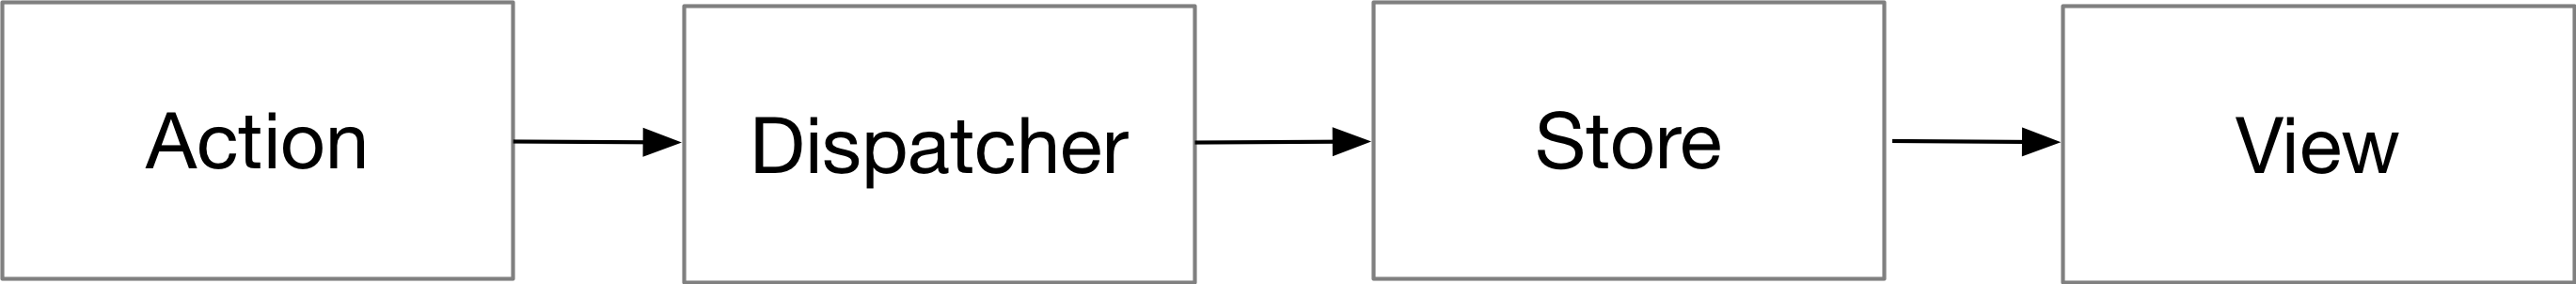
\includegraphics[scale=0.5]{bilder/grundlagen/UniDirection.png}
	\caption{Flux software architecture \cite{Flux}}
	\label{fig:FLUX}
\end{figure}

The dispatcher takes care of handling all actions and forwards them to the proper store.
The store holds the data and actions to change this data.
Once data was changed the store alerts all views that are affected by this data change, causing a re-rendering (see Fig. \ref{fig:FA}).

It is also possible that a view generates an action. This happens mainly through user interaction. This action is also passed to the dispatcher.

\begin{figure}[H]
	\centering
	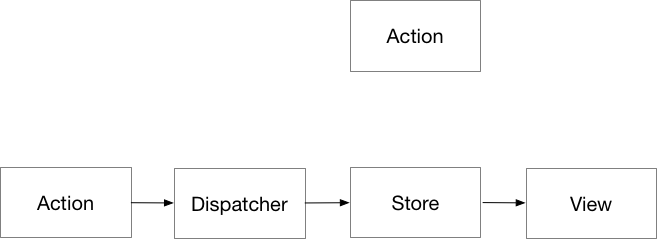
\includegraphics[scale=0.5]{bilder/grundlagen/uniDirection2.png}
	\caption{Flux with view action \cite{Flux}}
	\label{fig:FA}
\end{figure}

\subsubsection{Stores}
Stores contain the application state and the logic. 
Their role is similar to that of the model in the MVC,
but they can contain the state of several objects. 

Stores typically comprise the states of a domain within the application.
Stores register with the dispatcher with a callback function.
The callback has an action as a parameter.
A switch case based on the action type determines which method within the store should be executed.

In this way a store is updated by an action. As soon as the store is updated,
it reports that a state has changed so that all views can get the new state and update themselves.

\subsubsection{Dispatchers}
In the core of Flux lies the dispatcher. It is responsible for the control of the data flow within the application. In principle, it consists of a list of callbacks into the various stores.  It serves only to distribute the actions to the various stores. Each store registers itself with a dispatcher providing a callback . The dispatcher can also consider dependencies between different stores and control the order of the callbacks.

\subsubsection{Views and controller-views}

In React all views are composable and freely re-renderable. 
At the top of the view hierarchy there is a hidden view that listens to events that are sent by the store.
It is called a controller-view. 
The controller-view fetches the data from the store and passes it down to all descendants,
causing a re-rendering. Often the entire state of a store is passed down a chain of views allowing each descendant to take what it needs.

\subsubsection{Actions}

The dispatcher provides a dispatch method that has an action as a parameter. Actions can either be sent directly to the dispatcher or created via a creator function and sent to the dispatcher. The creation of an action usually takes place in the event handler of a view, for example due to a user interaction or a browser event.


\subsubsection{Conclusion}
The Flux architecture improves data consistency. 
The unidirectional data flow makes  applications based on Flux much easier to debug, 
since one can always follow easily the flow of actions. 
Furthermore, having the state and all logic updating the state in one place
it is also possible to do more meaningful unit tests.

\section{React and Flux}

The key framework used in this project is React, a  JavaScript library for developing user interfaces \cite{React}.

Back in 2011 Facebook noticed that it was getting hard to maintain
their application and to run it flawlessly, due to the  growing number of features.
Many people were hired and the team size expanded significantly.
With the growing team size it took longer to publish urgent updates.
Too many people were involved and concerns could not be separated in a satisfying manner.

A Facebook engineer called Jordan Walke decided to change that.
In the same year he created FlaxJs, a first prototype of React. 
Jordan was allowed to keep on working and created React in 2012. 

A short time later Instagram was bought by Facebook and both
companies agreed on using React as the new core technology for user experience.
 Further they agreed on making React publicly available. 

In early 2013 at JS ConfUS, React became an open source project. Facebook CEO Mark Zuckerberg, speaking on this conference said:  "Our biggest mistake was betting too much on HTML5". He promised to provide better experiences with React.

Currently React is getting increasingly popular. A trend analysis by Google shows that 
React is the leading modern user interface JavaScript framework (see Fig. \ref{fig:React}).

\begin{figure}[H]
	\centering
	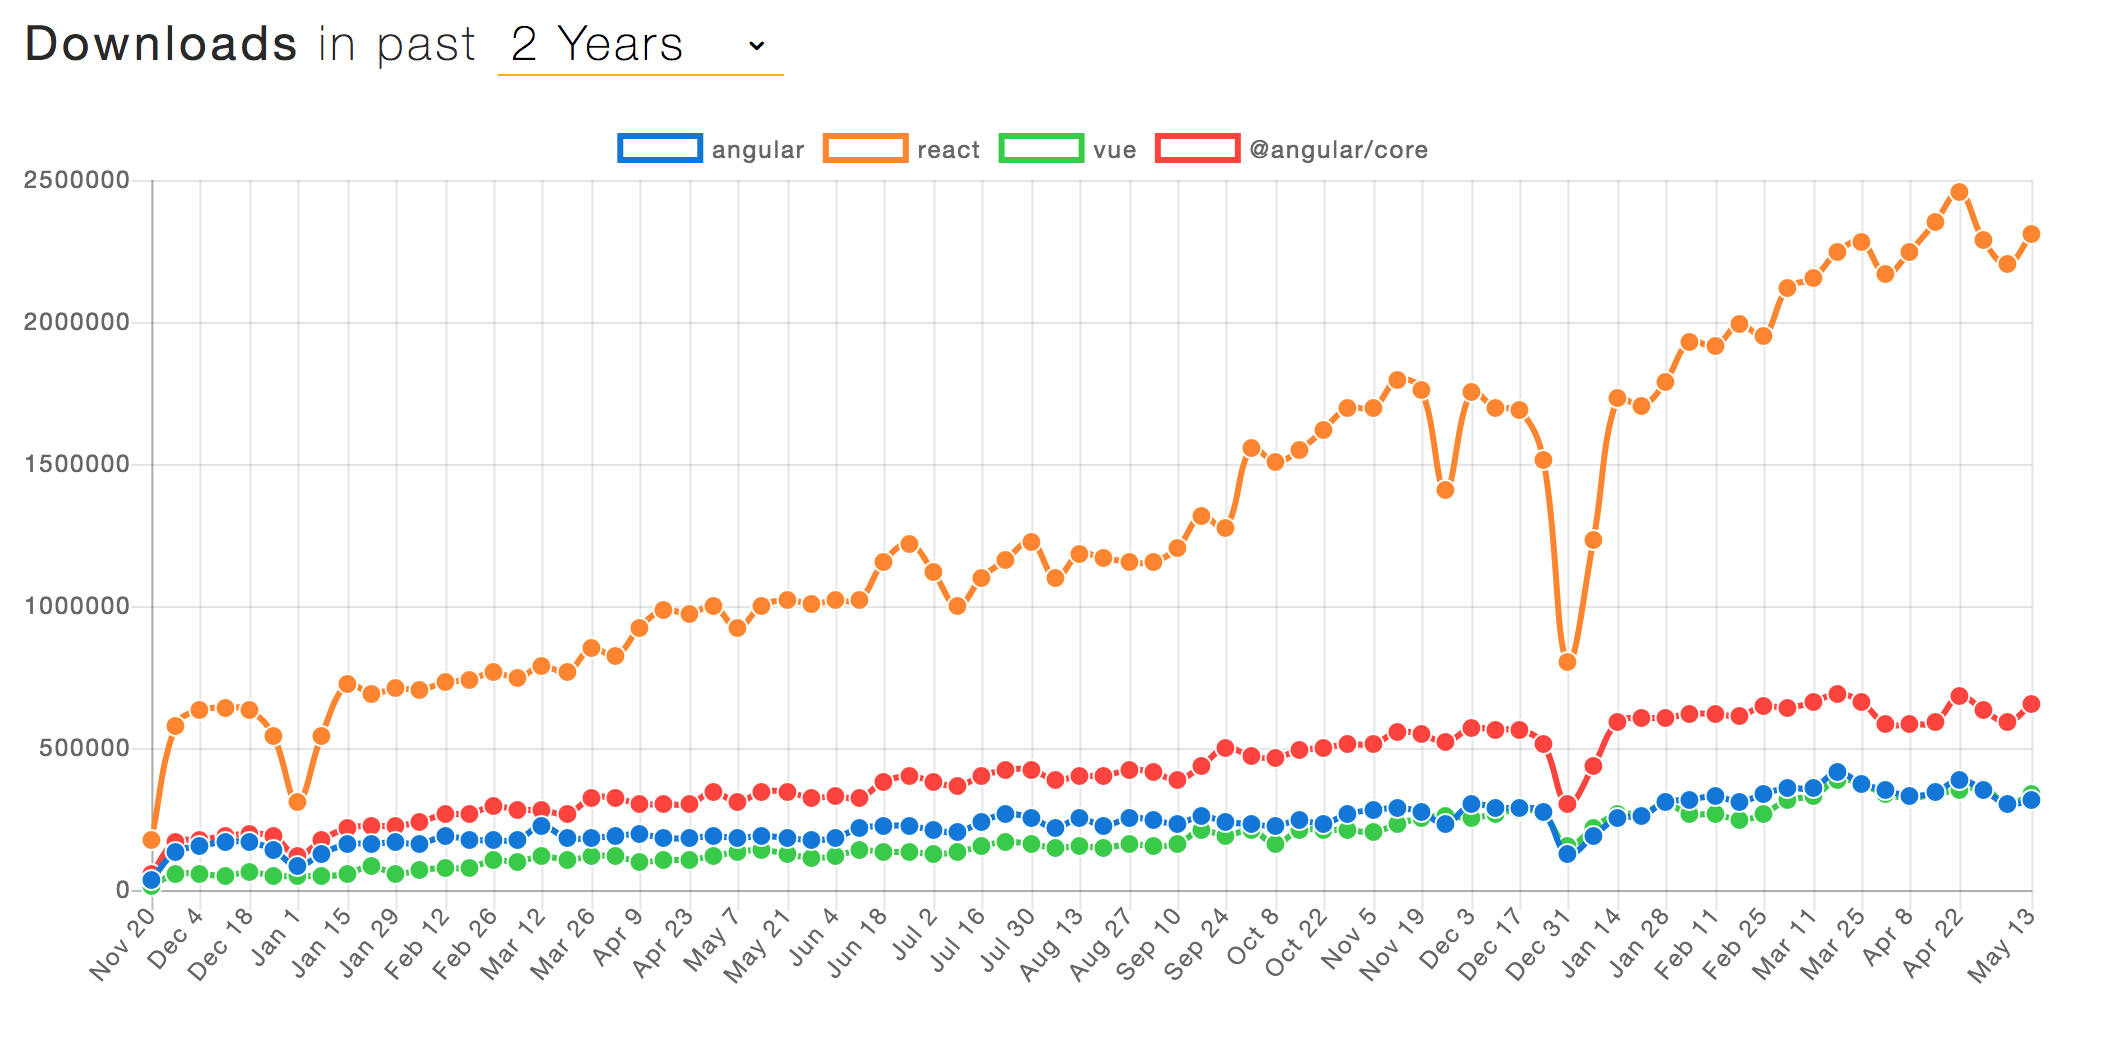
\includegraphics[scale=0.4]{bilder/grundlagen/ReactDownloads.png}
	\caption{Downloaded npm packages \cite{NPM}}
	\label{fig:React}
\end{figure}

This section is about analyzing how React is implementing the Flux software architecture. 
React is based on encapsulated components that manage their own state.
An application consists of nested components, somehow similar to the tree structure of an HTML DOM.

Components are written in JavaScript, so data can easily be passed through the application.
Any element that needs to be rendered is still written in HTML and parsed by React.
Each component has its own controllers.

In React, there are no HTML files decorated with special tags
but rather the HTML is generated from within JavaScript code.
Every component is fully standalone and testable on its own.
This makes React scalable and easy to test. There are no cascading dependencies.
Every time the state of a component changes,
the render function is called and the HTML is re-rendered with the changed data.
Components can be nested, for example a board game that consists of squares (see Fig. \ref{fig:Grid}).

\lstinputlisting[caption=Nested square component]{code/grundlagen/Component.js}

Each square is a component and part of the whole board game application.
There shall be a value assigned to the squares. Values are passed down to lower components via the 
"props" variable. 

\lstinputlisting[caption= Passing down variables with props]{code/grundlagen/ComponentWithProps.js}

\begin{figure}[H]
	\centering
	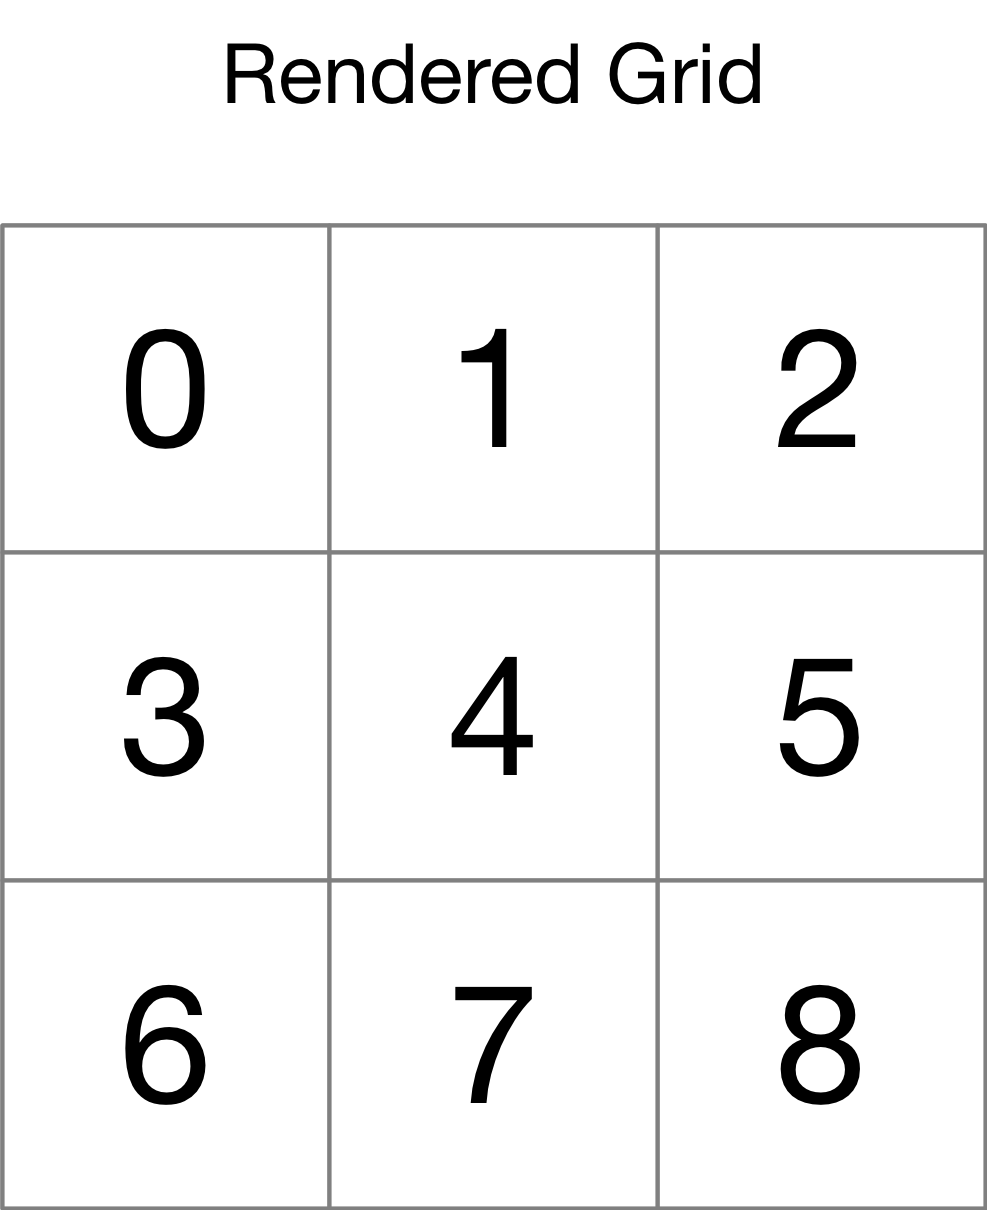
\includegraphics[width=0.3\linewidth]{bilder/grundlagen/GameGrid.png}
	\caption{Grid with numbers}
	\label{fig:Grid}
\end{figure}

Squares that have been clicked on shall show an 'X'. This value can be considered a local state.
It is definitely a private part of the square. First an initial state needs to be added.

\lstinputlisting[caption=Components with states]{code/grundlagen/ComponentWithState.js}

When \texttt{this.setState()} is called, an update is scheduled by React and the value is merged in the correct component state. Furthermore the component and all of its descendants are re-rendered. If a square was clicked it would now show an 'X' in the grid.

\subsection{Lifting state up}

Often data needs to be aggregated from multiple child components. 
Then it makes sense to lift all states up to a top-level component. 
The parent component  passes down the individual states to child components.

For example in a Tic Tac Toe game, to determine who has won 
the value of all square components would need to be checked. 
While that is technically feasible, a better approach is to save all states in the parent component.
The parent then checks the array in order to determine who has won.

The square component is no longer keeping its own state, it receives the value from its parent board. It informs the parent when it was clicked. Such components are called "controlled components" (see Fig. \ref{fig:TopLevel}).

\begin{figure}[H]
	\centering
	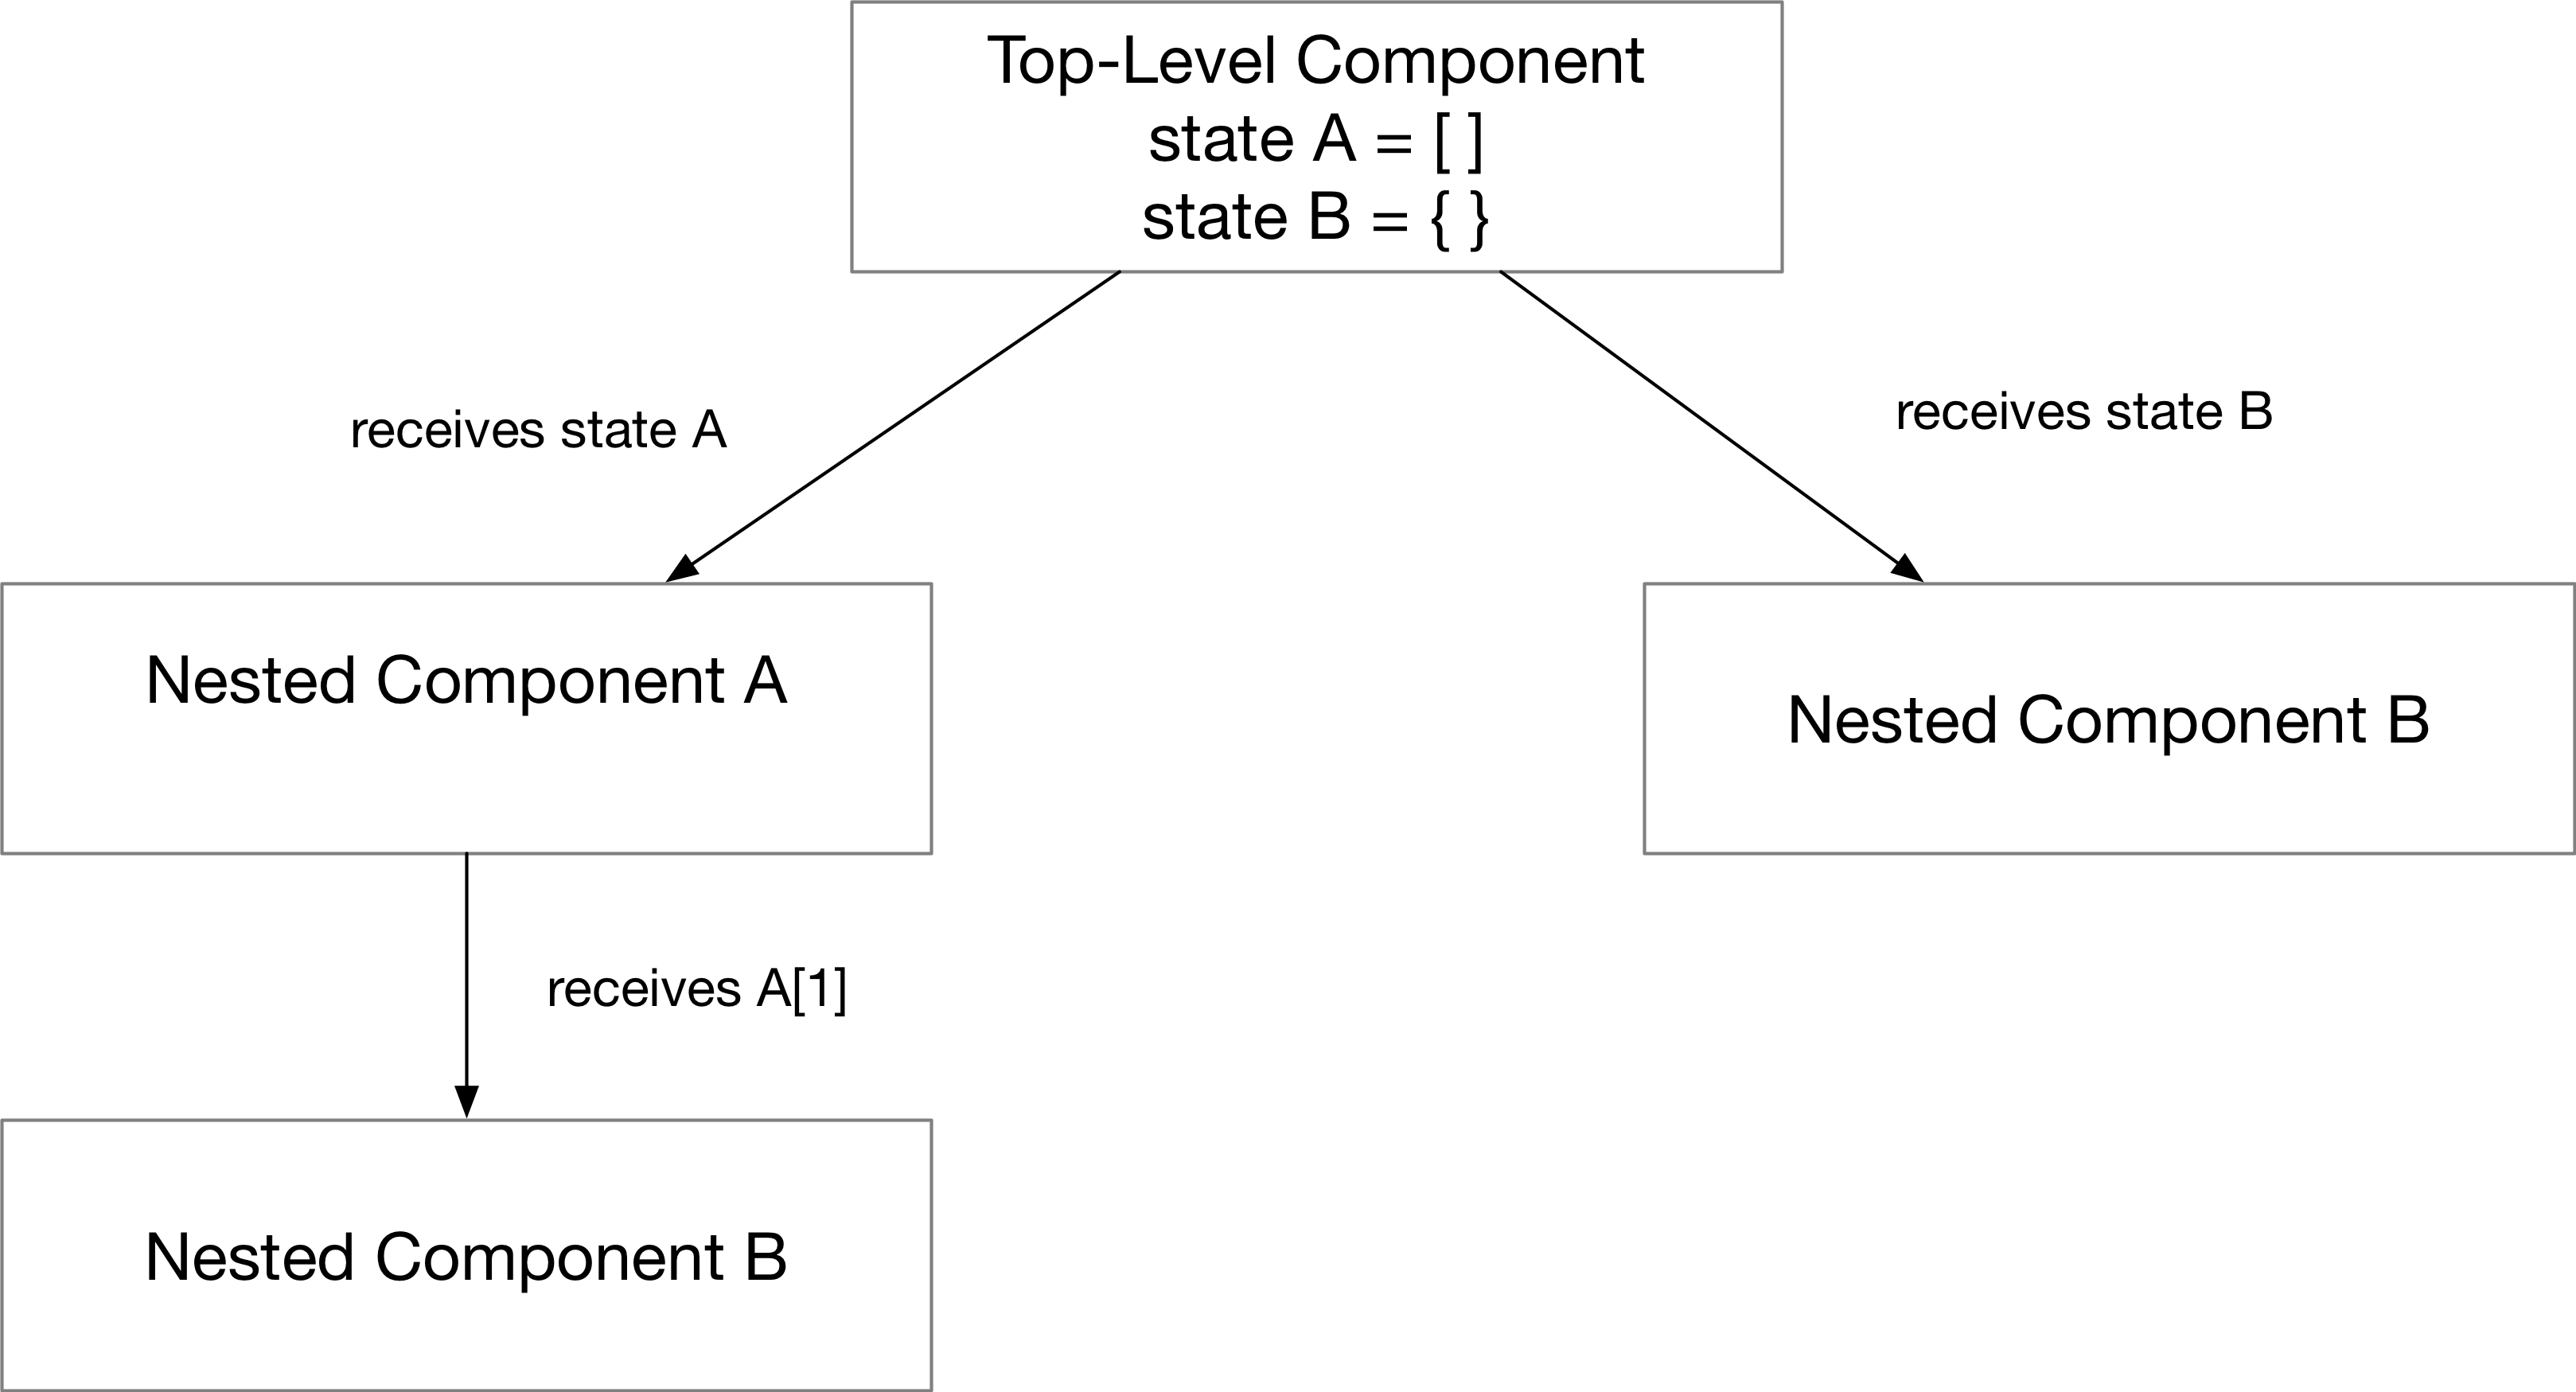
\includegraphics[width=1.0\linewidth]{bilder/grundlagen/topLevelComponent.png}
	\caption{Top-level component} 
	\label{fig:TopLevel}
\end{figure}


\subsection{Action- and dataflow}

Taking the last examples it is clear that data is only passed in one way, 
from the top-level component to a child component.
Another key principle is that actions are only passed up. 

For example if a nested component B is clicked or is triggered on a different event,  
some state B shall be changed in the top-level component. That is possible because 
all functions that change the data in the top-level component can be passed down 
to nested components via the \texttt{props} variable (see Fig. \ref{fig:DataFlow}).

\begin{figure}[H]
	\centering
	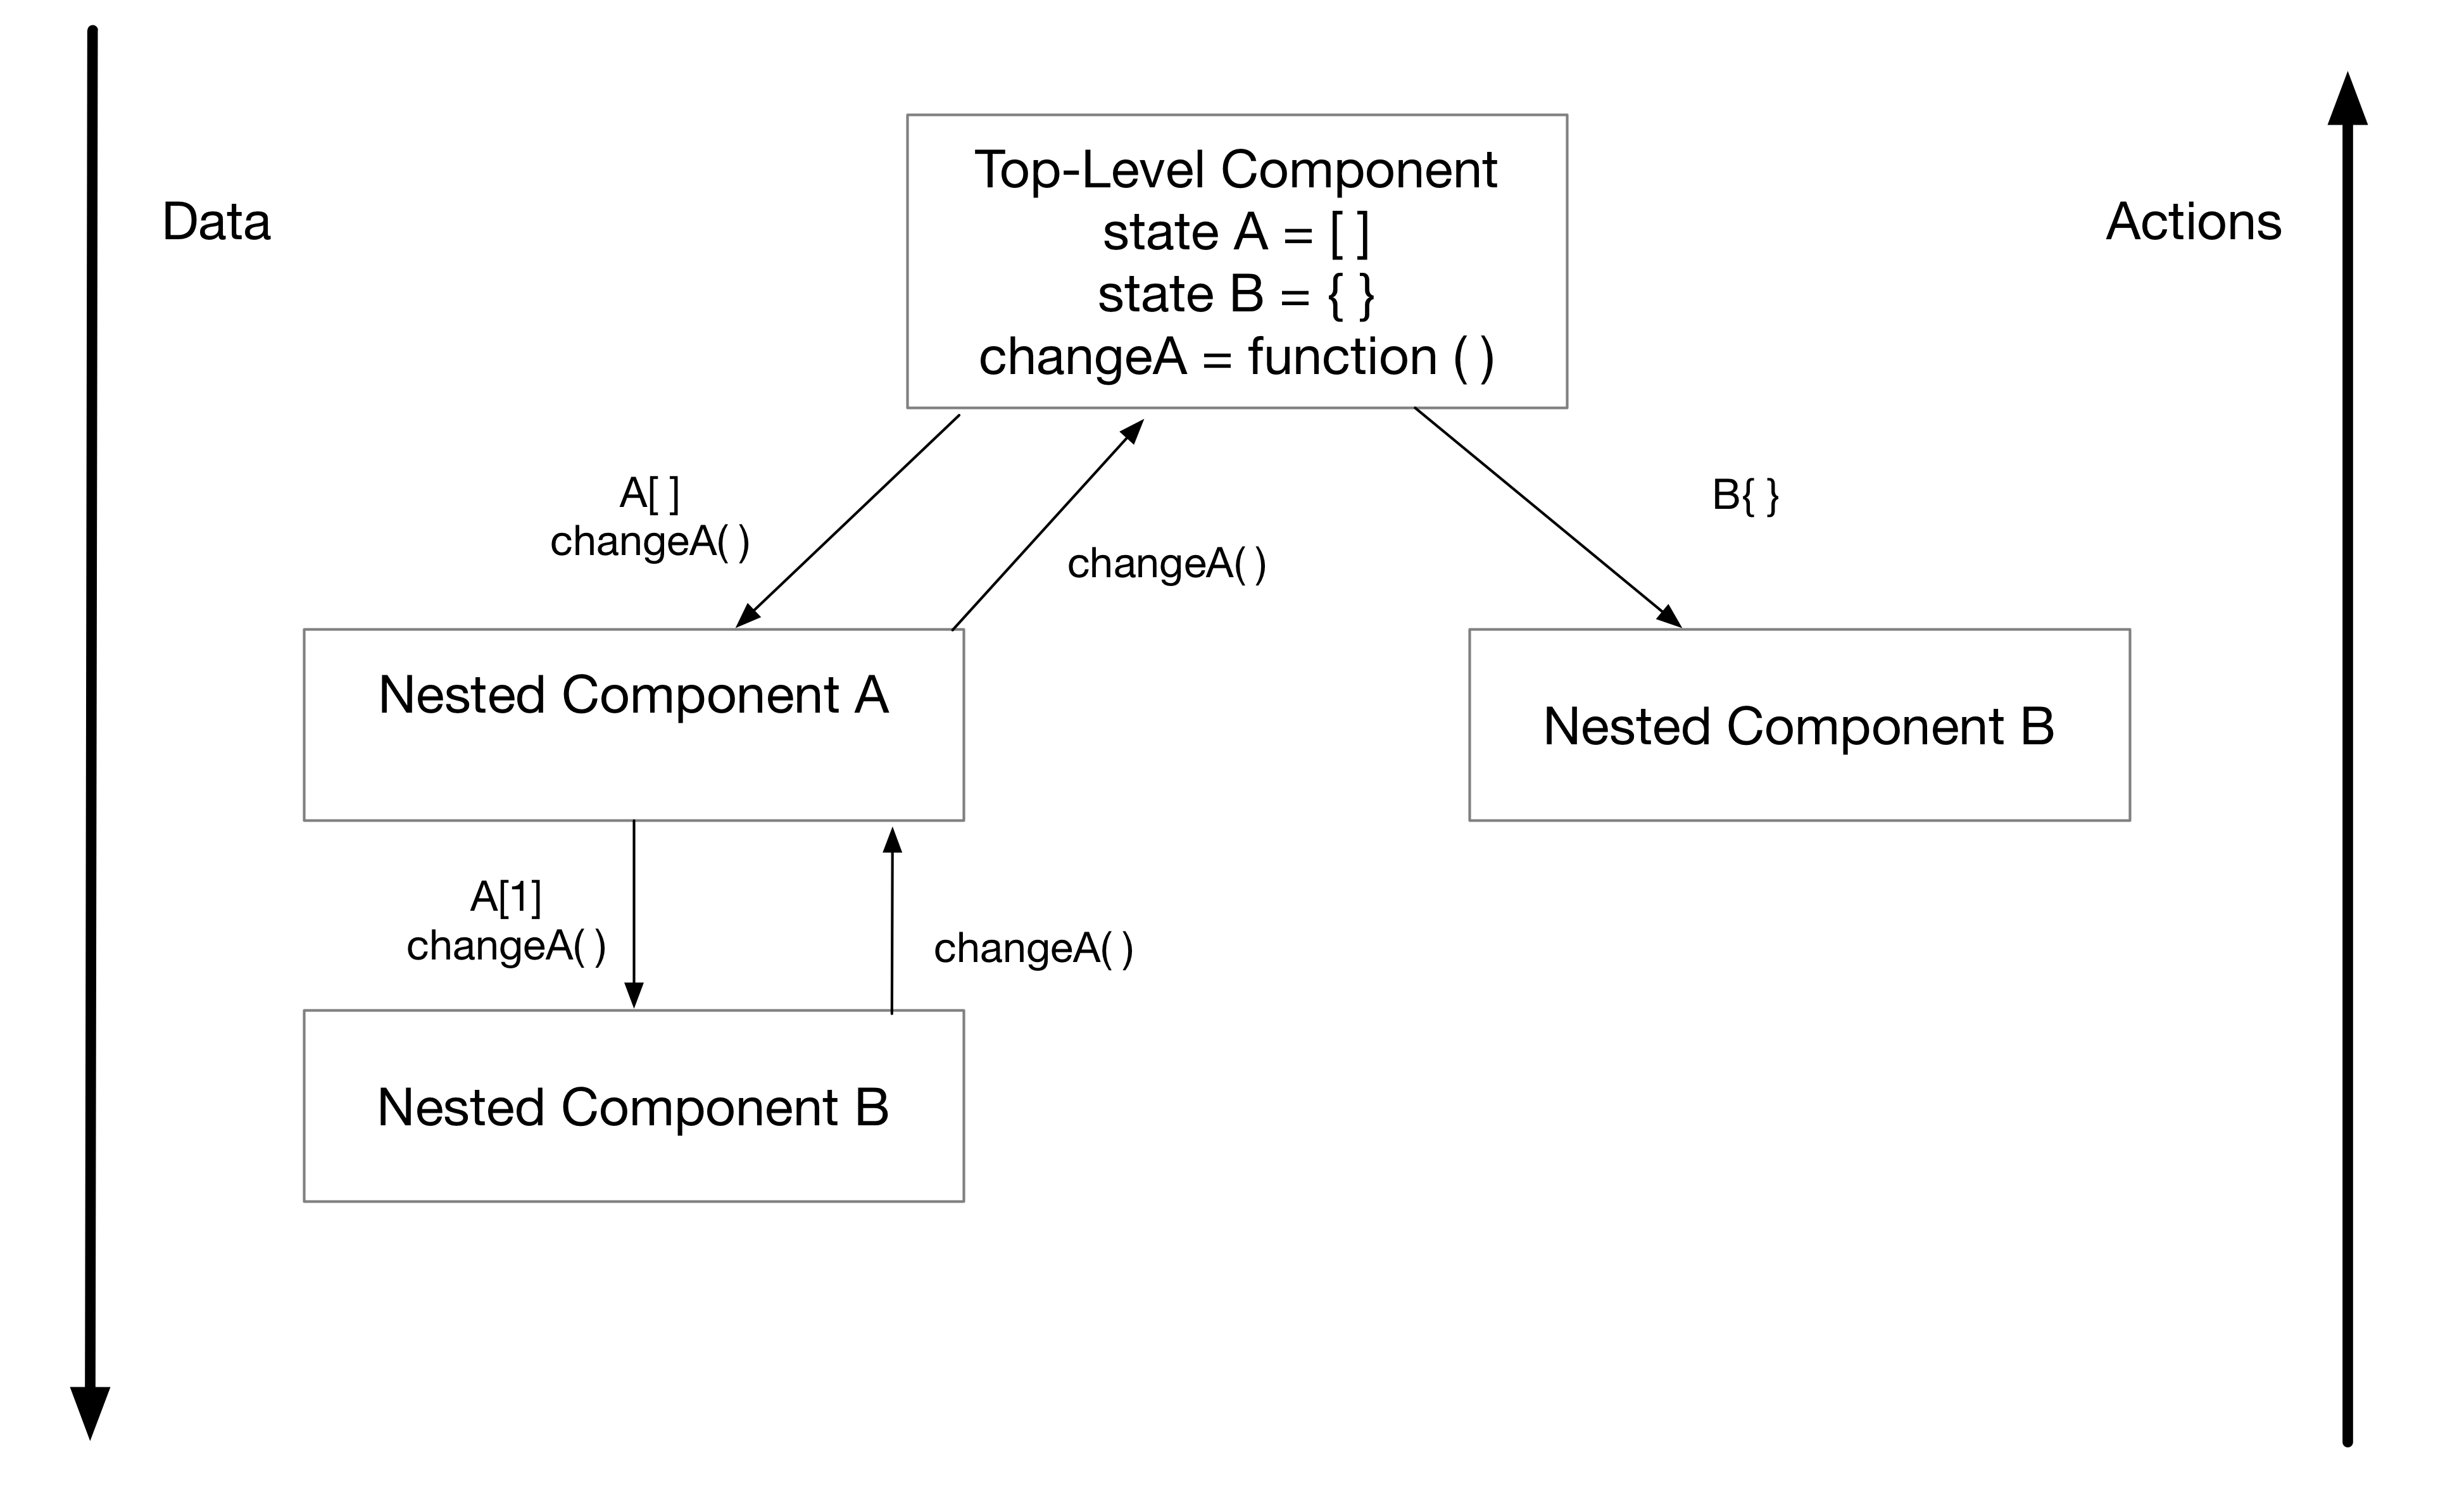
\includegraphics[width=1.0\linewidth]{bilder/grundlagen/dataFlow.png}
	\caption{Action- and dataflow}
	\label{fig:DataFlow}
\end{figure}


\subsection{High-order components}

As already known from the JavaScript introduction chapter
a high-level function can take another function as an argument.
Similar to that a high-order component is simply a high-order function
that takes a stateless component and returns the changed component. 
This makes it possible to add functionality to components on the fly. 

\lstinputlisting[caption=High-order component ]{code/grundlagen/hoc1.js}


\lstinputlisting[caption=Wrapped component]{code/grundlagen/hoc2.js}



\subsection{Virtual DOM}

Interactive web applications mainly consist of code that manipulate the DOM. 
Manipulating the HTML DOM is an expensive operation
since it often times results in unnecessary re-rendering of DOM elements.

For example changing one item in a list of ten items would lead to re-rendering all ten items.
React is addressing this problem by introducing a virtual DOM. 

The Virtual DOM is a replication of the HTML DOM but within JavaScript.
State changes lead to the creation of a new virtual DOM. React compares the new Virtual DOM with the previous one 
and just applies the differences between the two to the HTML DOM  (see Fig. \ref{fig:VirtualDom}).

\begin{figure}[H]
	\centering
	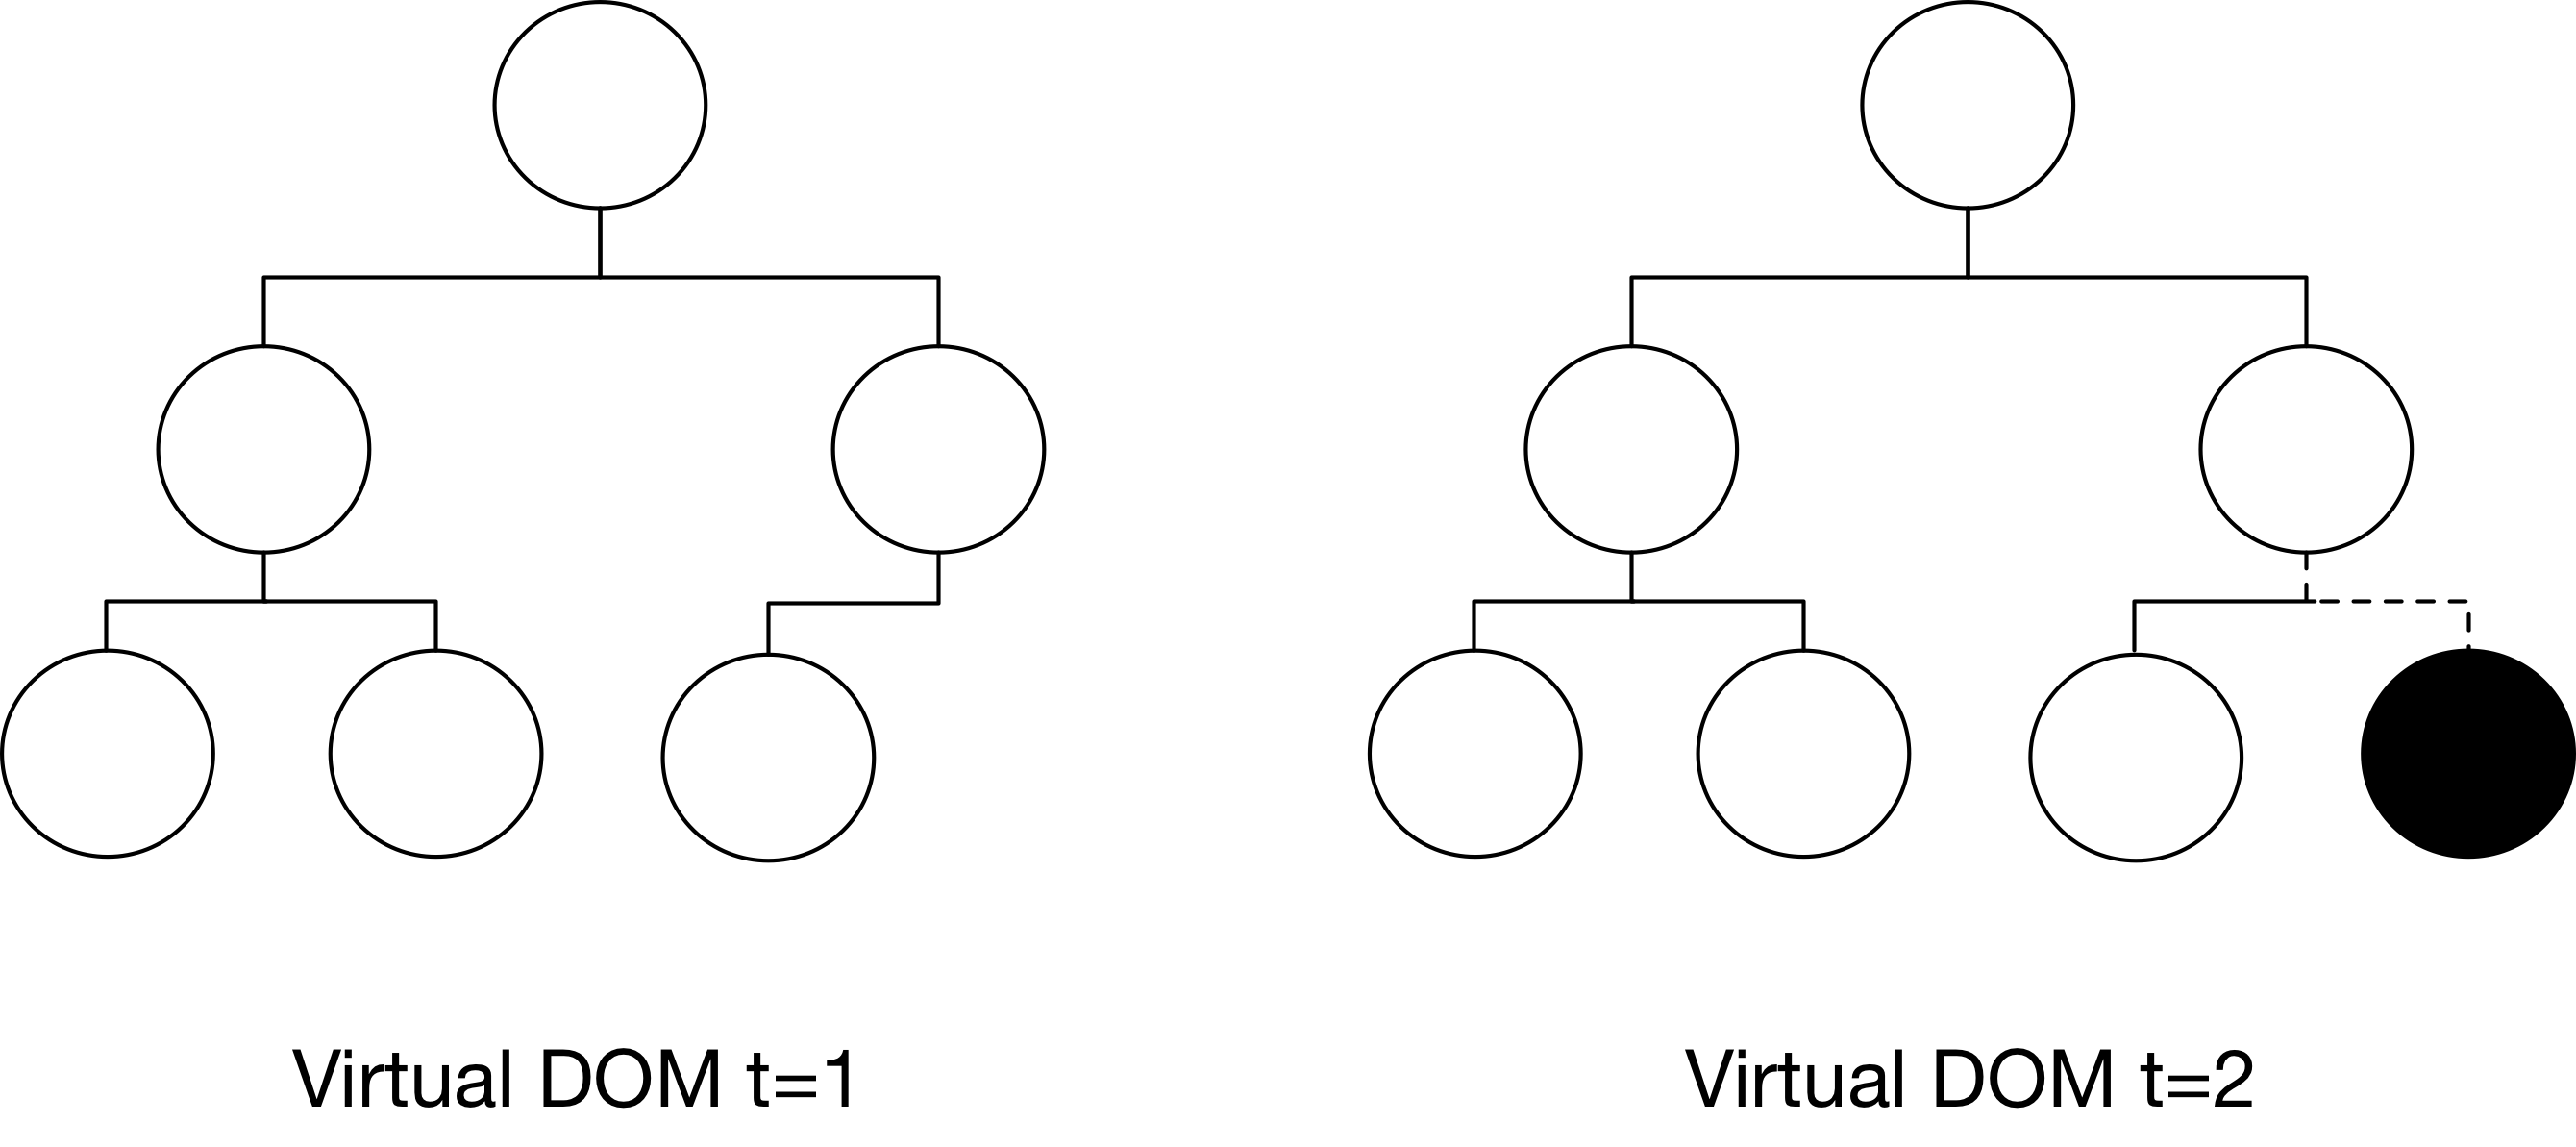
\includegraphics[width=0.8\linewidth]{bilder/grundlagen/VirtualDom.png}
	\caption{Virtual DOM comparison}
	\label{fig:VirtualDom}
\end{figure}

React is a relatively new framework with a new underlaying software architecture for user interfaces. This architecture leads to less files and more encapsulation. Therefore it scales better than classic MVC when having more views on the same data. Due to the Virtual DOM React is really performant when updating the DOM.

\subsection{Redux}

Redux evolves the ideas of the Flux software architecture.
This section is based on the official Redux guide \cite{Redux}.

The primary idea of Redux is to keep all states in a single store.
The only way the state may be changed is by emitting actions.
Actions are objects describing what happened, either at the user interface or at 
the client server interface. So called "pure reducer" functions
define how actions change the state tree.

The major difference between Flux and Redux is that Redux does not have 
a dispatcher and does not support more than one store. With a single root reducer there is just a single store.
In larger applications the root reducer can be split into several reducers,
each operating independently on different parts of the state tree.
 
Redux adds a lot of overhead to an application, more files and code are created. 
Considering that, Redux should only be used if the following points apply.

\begin{itemize}
\item A considerable amount of data is changing over time
\item A single source of truth is needed (all states in one place)
\item Keeping all of the states in a top-level component is no longer sufficient
\end{itemize}

It should further be mentioned that Redux destroys a key principle of React by 
providing access to the state from all components in an application directly. 
It is no longer obvious what data is used in which component (see Fig. \ref{fig:Redux}).
\begin{figure}[H]
	\centering
	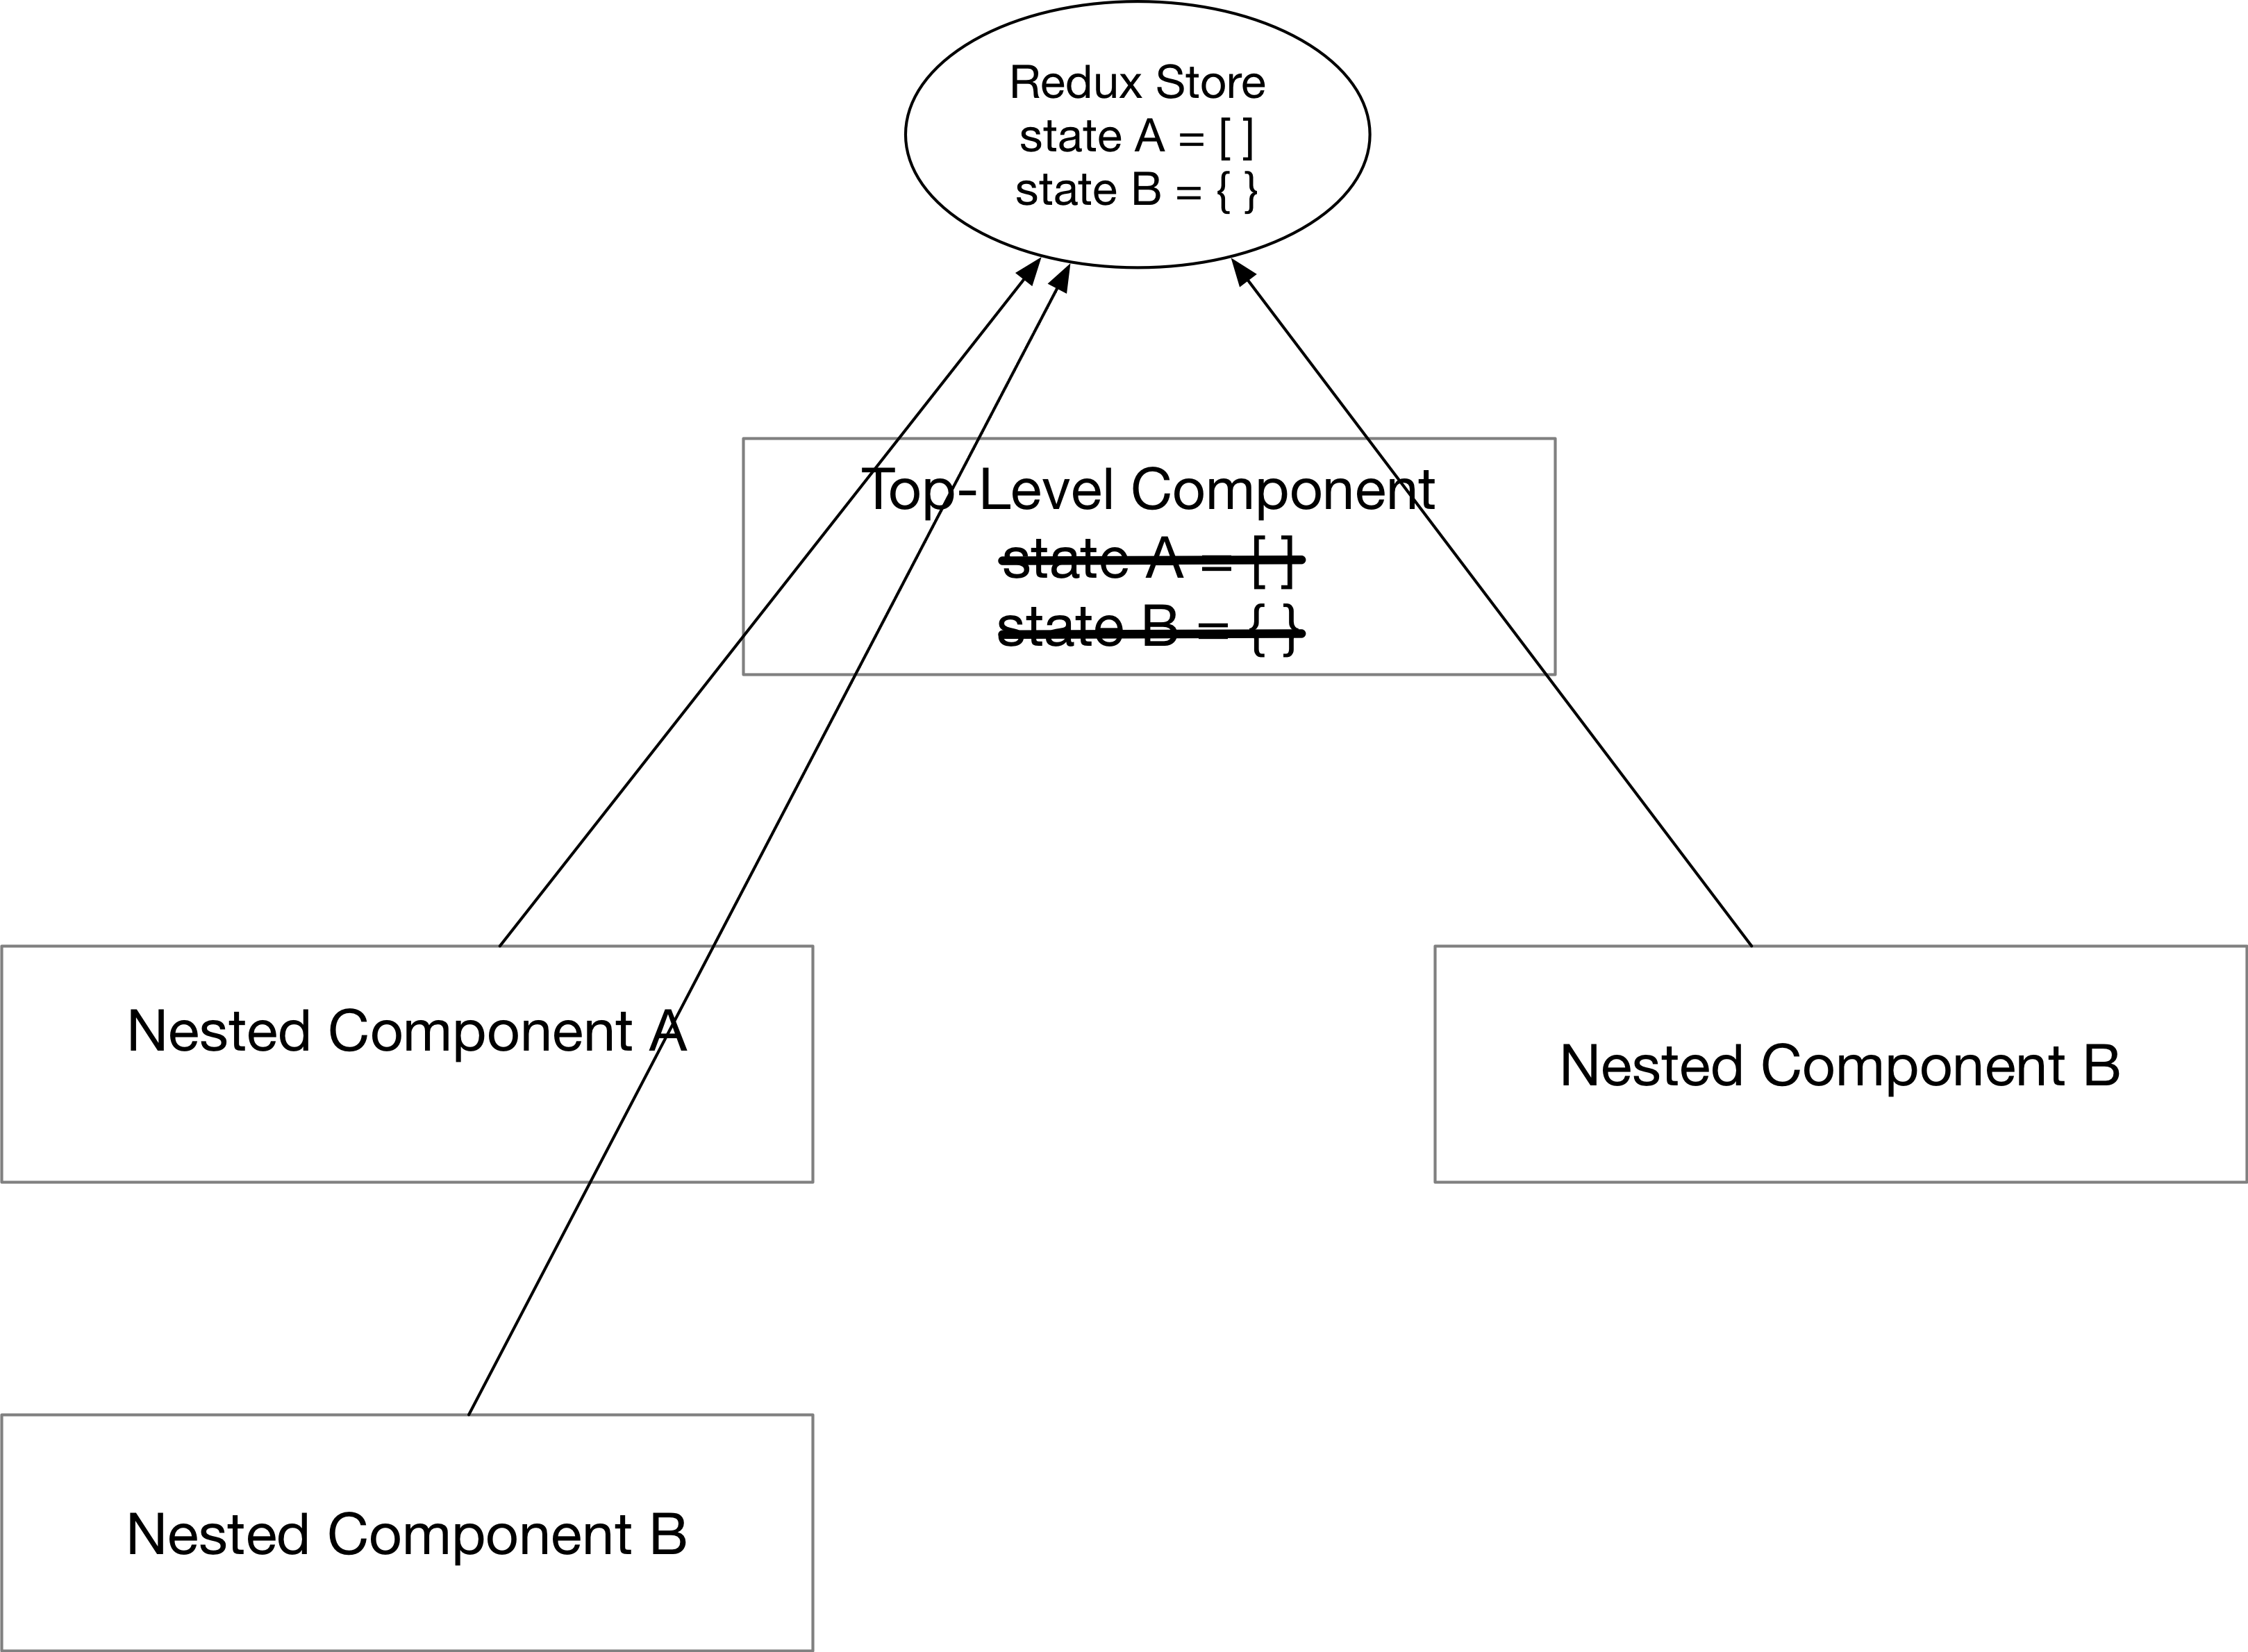
\includegraphics[width=0.8\linewidth]{bilder/grundlagen/reduxStore.png}
	\caption{Redux store}
	\label{fig:Redux}
\end{figure}

\section{TensorFlow.js}
TensforFlow.js is an open source JavaScript library for training and deploying
neural networks in a browser and on Node.js. 
First introduced in Spring 2018 it already provides intuitive APIs to build and train models from scratch in a browser.
Existing models can be loaded and re-trained.
Normal TensorFlow models can be imported and used. 

TensorFlow is computation intensive.
It can be significantly accelerated by accessing graphic processors via a WebGl interface.
This facilitates to train a network and execute predictions in a reasonable time. 
In the following we will discuss some core concepts of TensorFlow.js \cite{TenosrFLowJs}. 

\subsection{Core Concepts}

Tensors are sets of numbers with an additional shape attribute.
The shape attribute defines the tensors dimensions, 
in other words how to interpret the set as a numerical array.
Tensors are immutable, the values of a tensor can not be changed.

\lstinputlisting{code/grundlagen/tensor.js}

It is possible to create variables from tensors. Such variables have the same structure as the tensor but they 
are mutable.

\lstinputlisting{code/grundlagen/variables.js}

Tensors provide operations that can be performed on them. In TensorFlow.js there is a wide variety
of algorithms that can be applied to tensors.
These operations do not change a tensor, instead they create new tensors.

\lstinputlisting{code/grundlagen/operations.js}

TensorFlow.js models are comparable  to functions as they  take inputs and produce outputs.
TensorFLow.js provides a high-level API called \texttt{f.model()} to construct a model with layers.

\lstinputlisting{code/grundlagen/model.js}

\subsection{Performance}

Even though TensorFlow.js can access the local graphics processing unit (GPU), 
the Tensorflow.js development team reports that TensorFlow implementations 
written in Pyhton or C++ perform 1.5 to 2 times faster.
Small models seem to train faster in the browser, but larger models will 
perform 10-15 faster in Python than on JavaScript \cite{TenosrFLowJs}.

\subsection{Summary}
TensorFLow.js makes constructing neural networks, training and predicting quite easy.
With GPU support such networks run relatively fast even in JavaScript, although 
they are not as performant as TensorFlow distributions
written in C++ or Python. 

TensorFlow.js  distributes the computational load 
across many computers and thereby scales much better than if an algorithm would be running on a single
server, even if that was very performant.
